\documentclass[spanish]{beamer}
\usetheme{metropolis}

%\usefonttheme[onlymath]{serif}
\usepackage{hyperref}
\hypersetup{
	colorlinks=true,
	urlcolor=blue,
	linkcolor=magenta,
	citecolor=blue,
}
\usepackage{tikz}
\usepackage{tikz-cd}
\usepackage{mathtools}

\makeatletter
\newenvironment<>{proofs}[1][\proofname]{%
	\par
	\def\insertproofname{#1\@addpunct{.}}%
	\usebeamertemplate{proof begin}#2}
{\usebeamertemplate{proof end}}
\makeatother

\theoremstyle{definition}
\renewcommand{\proofname}{Demostración}

\newtheorem*{defn}{Definición}
\newtheorem*{lema}{Lema}
\newtheorem*{obs}{Observación}
\newtheorem*{teo}{Teorema}
\newtheorem*{prop}{Proposición}
\newtheorem*{coro}{Corolario}
\newtheorem*{af}{Afirmación}
\newtheorem*{ejer}{Ejercicio}
\newtheorem*{ejem}{Ejemplo}
\newtheorem*{pregunta}{Pregunta}

\newcommand{\R}{\mathbb{R}}
\newcommand{\Z}{\mathbb{Z}}
\newcommand{\N}{\mathbb{N}}
\newcommand{\C}{\mathbb{C}}
\newcommand{\Q}{\mathbb{Q}}
\newcommand{\Hy}{\mathbb{H}}
\newcommand{\A}{\mathbb{A}}
\newcommand{\D}{\mathbb{D}}
\newcommand{\M}{\mathbb{M}}
\DeclareMathOperator{\Id}{Id}
\DeclareMathOperator{\img}{img}
\DeclareMathOperator{\rel}{rel}
\DeclareMathOperator{\Mod}{Mod}
\DeclareMathOperator{\Hom}{Hom}
\DeclareMathOperator{\Homeo}{Homeo}
\DeclareMathOperator{\Isom}{Isom}
\DeclareMathOperator{\Deck}{Deck}
\DeclareMathOperator{\Diff}{Diff}
\DeclareMathOperator{\SL}{SL}
\DeclareMathOperator{\PSL}{PSL}
\DeclareMathOperator{\SMod}{SMod}
\DeclareMathOperator{\LMod}{LMod}
\DeclareMathOperator{\PMod}{PMod}
\DeclareMathOperator{\SHomeo}{\mathcal{S}Homeo}
\DeclareMathOperator{\LHomeo}{\mathcal{L}Homeo}

\usepackage[style=mla,backend=bibtex]{biblatex}
\addbibresource{bir-bib.bib}

\title{Aplicaciones a presentaciones del grupo modular}
\date{}
\author{Daniel González Casanova Azuela}

\begin{document}
	\maketitle
	\begin{frame}{Plan de la charla}
		\begin{enumerate}
			\item Definiciones.
			\item Algunos resultados que necesitaremos.
			\item Una presentación de $\Mod(S_2)$.
			\item Generalización para $\SMod(S_g)$.
			\item Aplicación a la signatura de una 4-variedad.
			\item Aplicación a la comohomología en dimensiones bajas de $\SMod(S_g)$.
		\end{enumerate}
	\end{frame}

	\section{Preliminares\\
	{\small Definiciones}}
	\begin{frame}{Definiciones}
	\begin{enumerate}
	\item El \textbf{\textit{mapping class group}} $\Mod(S_{g,n})$ de una superficie cerrada, orientable de género $g$ con $n$ puntos marcados $S_{g,n}$ es el grupo de clases de homotopía de homeomorfismos que preservan la orientación, la frontera y el conjunto de puntos marcados. \pause (Las homotopías también preservan la frontera y los puntos marcados.)
\end{enumerate}
	\end{frame}
	
		\begin{frame}{Definiciones}
		\begin{enumerate}
	\item[2.] \begin{itemize}
		\item Una función $p:S\to X$ es un \textbf{\textit{cubriente ramificado}} si existe un conjunto finito $B\subseteq X$ tal que la restricción $S\backslash p^{-1}(B)\to X\backslash B$ es un cubriente. \pause
	
	\item El \textbf{\textit{grado}}  de $p$ es $d$ si el grado del cubriente asociado es $d$. \pause
	
	\item Los \textbf{\textit{puntos de ramificación}} son puntos con menos preimágenes que $d$. \pause
	
	\item Decimos que $p$ es \textbf{\textit{regular}} si el grupo de transformaciones de cubierta actúa transitivamente en $S$.
	\end{itemize}
		\end{enumerate}
	\end{frame}
	
	\begin{frame}{Definiciones}
		\begin{enumerate}
	\item[3.] Decimos que un grupo finito $G$ es \textbf{\textit{soluble}} si tiene una \textbf{\textit{serie normal}}
\[G=G_0\geq G_1\geq G_2\geq\cdots\geq G_t=\{1\}\]
cuyos \textbf{\textit{grupos factores}}
\[G_0/G_1,G_1/G_2,\ldots,G_{n-1}/G_n\]
son abelianos.

		\end{enumerate}
	\end{frame}
	
		\begin{frame}{Definiciones}
		\begin{enumerate}
			\item[4.] El grupo de \textbf{\textit{transformaciones de cubierta}} de un cubriente $p$ es ${\operatorname{Deck}(p)=\{h:S\overset{\text{homeo}}{\longrightarrow} S\;|p=hp\}}$.
			\[\begin{tikzcd}[ampersand replacement=\&, column sep=tiny]
				S\arrow[rr,"h"]\arrow[rd,"p",swap]\&\&S\arrow[ld,"p"]\\
				\&X
			\end{tikzcd}\]
			\pause Decimos que $p$ es un \textbf{\textit{cubriente soluble}} si $\Deck(p)$ es soluble.
			
		\end{enumerate}
	\end{frame}
	
			\begin{frame}{Definiciones}
		\begin{enumerate}
			\item[5.]  Un homeomorfismo $f:X\to X$ se \textbf{\textit{levanta}} a $\tilde{f}:S\to S$ si $p\tilde{f}= pf$ para cualquier punto de $S$.
			\[\begin{tikzcd}[ampersand replacement=\&]
				S\arrow[r,"\tilde{f}"]\arrow[d,"p",swap]\&S\arrow[d,"p"]\\
				X\arrow[swap,r,"f"]\&X
			\end{tikzcd}\]
			
			\pause$\LMod(X)$ es el subgrupo de clases de equivalencia en $\Mod(X)$ que tienen un representante que se levanta a $S$. \pause Recordemos que $fp$ se levanta a $\tilde{f}$ si y sólo si $(fp)_*\pi_1(S)\subset p_*\pi_1(S)$.
			
		\end{enumerate}
	\end{frame}
	
	\begin{frame}{Definiciones}
		\begin{enumerate}
			\item[6.]  \begin{itemize}
				\item Una función $\tilde{f}:S\to S$ \textbf{\textit{preserva fibras}} si para cualquier $x\in X$ existe $y\in X$ tal que $\tilde{f}(p^{-1}(x))=p^{-1}(y)$ como conjuntos, es decir, $\tilde{f}$ manda fibras en fibras.
			
			\pause \item $\SMod(S)$ es el subgrupo de clases de equivalencia en $\Mod(S)$ que tienen un representante que preserva fibras (la homotopía puede no preservar fibras). \pause Son exactamente los levantamientos de los homeomorfismos levantables.
			\end{itemize}
			
		\end{enumerate}
	\end{frame}
	
		\begin{frame}{Definiciones}
		\begin{enumerate}
			\item[7.] El \textbf{\textit{mapping class group puro $\PMod(S_{g,n})$}} es el subgrupo de $\Mod(S_{g,n})$ que consiste de los elementos que fijan cada punto marcado individualmente.\pause
			
			\item[8.]  Decimos que $p$ tiene la \textbf{\textit{propiedad de Birman-Hilden}} si para cualesquiera dos homeomorfismos homotópicos que preservan fibras hay una homotopía entre ellos que preserva fibras.
			
		\end{enumerate}
	\end{frame}
	
		\section{Preliminares\\
		{\small Teorema de Birman-Hilden}}
	
	\begin{frame}{Teorema de Birman-Hilden}
		\begin{teo}[Birman-Hilden]
			
			Sea $p:S\to X$ un cubriente regular ramificado con un número finito de hojas donde $S$ es una superficie hiperbólica. Supongamos que $p$ o bien no es ramificado o bien es soluble. Entonces $p$ tiene la propiedad de Birman-Hilden.
		\end{teo}
	\end{frame}
	
	\begin{frame}{Equivalencias del teorema de Birman-Hilden}
		\begin{prop}\leavevmode
			
			Sea $p:S\to X$ un cubriente regular ramificado con un número finito de hojas donde $S$ es una superficie hiperbólica sin frontera. Las siguientes son equivalentes:
			\begin{enumerate}[(i)]
				\item $p$ tiene la propiedad de Birman-Hilden.
				\item El mapeo natural $\LMod(X)\to\SMod(S)/D$ es inyectivo.
				\item El mapeo natural $\SMod(S)\to\LMod(X)$ está bien definido.
				\item $\SMod(S)/D\cong\LMod(X)$.
			\end{enumerate}
			donde $D$ son las clases de homotopía de transformaciones de cubierta de $S$.
			%(es decir, los levantamientos de la identidad, y por lo tanto el kernel del mapeo natural $\LMod(X)\to\SMod(S)$).
		\end{prop}
	\end{frame}
	
	\begin{frame}{Equivalencias del teorema de Birman-Hilden}
		\begin{enumerate}[(i)]\tiny
			\item $p$ tiene la propiedad de Birman-Hilden.
			\item El mapeo natural $\LMod(X)\to\SMod(S)/D$ es inyectivo.
			\item El mapeo natural $\SMod(S)\to\LMod(X)$ está bien definido.
			\item $\SMod(S)/D\cong\LMod(X)$
			\vspace{2pt}
			
			donde $D$ son las clases de homotopía de transformaciones de cubierta de $S$.
		\end{enumerate}
		\begin{proofs}\leavevmode
			
			Primero simplemente observemos que el mapeo $\LMod(X)\to\SMod(S)$ siempre está bien definido por la propiedad del levantamiento de homotopías:
			
			\[\begin{tikzcd}[ampersand replacement=\&]
				\&\& S\arrow[d,"p"]\\
				S\arrow[dashed,urr,"\textcolor{cyan}{\widetilde{fp}}\simeq\textcolor{magenta}{\widetilde{gp}}"]\arrow[r,swap,"p"]\& X\arrow[r,swap,"\textcolor{cyan}{f}\simeq\textcolor{magenta}{g}"]\& X
			\end{tikzcd}\]
		\end{proofs}
	
	\end{frame}
	
	\begin{frame}{Equivalencias del teorema de Birman-Hilden}
		\begin{enumerate}[(i)]\tiny
			\item $p$ tiene la propiedad de Birman-Hilden.
			\item El mapeo natural $\LMod(X)\to\SMod(S)/D$ es inyectivo.
			\item El mapeo natural $\SMod(S)\to\LMod(X)$ está bien definido.
			\item $\SMod(S)/D\cong\LMod(X)$
			\vspace{2pt}
			
			donde $D$ son las clases de homotopía de transformaciones de cubierta de $S$.
		\end{enumerate}
		\begin{proof}\leavevmode
			
		Observemos también que las transformaciones de cubierta son levantamientos de la identidad.
					\[\begin{tikzcd}[ampersand replacement=\&]
			\&\& S\arrow[d,"p"]\\
			S\arrow[dashed,urr,"\textcolor{magenta}{\widetilde{\Id}}"]\arrow[r,swap,"p"]\& X\arrow[r,swap,"\textcolor{magenta}{\Id}"]\& X
		\end{tikzcd}\]
		\end{proof}
		
	\end{frame}
	
	\begin{frame}{Equivalencias del teorema de Birman-Hilden}
		\begin{enumerate}[(i)]\tiny
			\item $p$ tiene la propiedad de Birman-Hilden.
			\item El mapeo natural $\LMod(X)\to\SMod(S)/D$ es inyectivo.
			\item El mapeo natural $\SMod(S)\to\LMod(X)$ está bien definido.
			\item $\SMod(S)/D\cong\LMod(X)$
			\vspace{2pt}
			
			donde $D$ son las clases de homotopía de transformaciones de cubierta de $S$.
		\end{enumerate}
		\begin{proofs}\leavevmode
			
			(i)$\implies$(ii) Tomamos el neutro en $\SMod(S)/D$ y mostramos que su única preimagen es el neutro en $\LMod(X)$. En efecto, si $\textcolor{cyan}{\widetilde{fp}}\simeq\textcolor{magenta}{\tilde{\Id}}$, por (i) la homotopía preserva fibras, desciende al cociente y obtenemos que $\textcolor{cyan}{f}\simeq\textcolor{magenta}{\Id}$.
			
			\[\begin{tikzcd}[ampersand replacement=\&]
				\&\& S\arrow[d,"p"]\\
				S\arrow[dashed,urr,"\textcolor{cyan}{\widetilde{fp}}\simeq\textcolor{magenta}{\widetilde{\Id}}"]\arrow[r,swap,"p"]\& X\arrow[r,swap,"\textcolor{cyan}{f}\simeq\textcolor{magenta}{\Id}"]\& X
			\end{tikzcd}\]
		\end{proofs}
	\end{frame}
	
		\begin{frame}{Equivalencias del teorema de Birman-Hilden}
		\begin{enumerate}[(i)]\tiny
			\item $p$ tiene la propiedad de Birman-Hilden.
			\item El mapeo natural $\LMod(X)\to\SMod(S)/D$ es inyectivo.
			\item El mapeo natural $\SMod(S)\to\LMod(X)$ está bien definido.
			\item $\SMod(S)/D\cong\LMod(X)$
			\vspace{2pt}
			
			donde $D$ son las clases de homotopía de transformaciones de cubierta de $S$.
		\end{enumerate}
		\begin{proofs}\leavevmode
			
			(ii)$\implies$(iii) En el siguiente diagrama
			\[\begin{tikzcd}[ampersand replacement=\&]
				\&\SMod(S)\arrow[d,"\pi"]\arrow[ld,dashed]\\
				\LMod(X)\arrow[r,leftrightarrow,swap,"\text{(ii)}"]\&\SMod(S)/D
			\end{tikzcd}\]
			la flecha punteada es el mapeo natural.
			
		\end{proofs}
	\end{frame}
		
	\begin{frame}{Equivalencias del teorema de Birman-Hilden}
			\begin{enumerate}[(i)]\tiny
				\item $p$ tiene la propiedad de Birman-Hilden.
				\item El mapeo natural $\LMod(X)\to\SMod(S)/D$ es inyectivo.
				\item El mapeo natural $\SMod(S)\to\LMod(X)$ está bien definido.
				\item $\SMod(S)/D\cong\LMod(X)$
				\vspace{2pt}
				
				donde $D$ son las clases de homotopía de transformaciones de cubierta de $S$.
			\end{enumerate}
			\begin{proofs}\leavevmode
				
				(iii)$\implies$(i)  Supongamos que  $\textcolor{cyan}{\widetilde{fp}}\simeq\textcolor{magenta}{\widetilde{gp}}$ y veamos que hay una homotopía que preserva fibras. Que el mapeo natural esté bien definido implica que $\textcolor{cyan}{f}\simeq\textcolor{magenta}{g}$, y por la propiedad del levantamiento las funciones de en medio se levantan.
				
				\[\begin{tikzcd}[ampersand replacement=\&]
					\&\& S\arrow[d,"p"]\\
					S\arrow[dashed,urr,"\textcolor{cyan}{\widetilde{fp}}\simeq\textcolor{magenta}{\widetilde{gp}}"]\arrow[r,swap,"p"]\& X\arrow[r,swap,"\textcolor{cyan}{f}\simeq\textcolor{magenta}{g}"]\& X
				\end{tikzcd}\]
			\end{proofs}
			
		\end{frame}

		
	\begin{frame}{Equivalencias del teorema de Birman-Hilden}
		\begin{enumerate}[(i)]\tiny
			\item $p$ tiene la propiedad de Birman-Hilden.
			\item El mapeo natural $\LMod(X)\to\SMod(S)/D$ es inyectivo.
			\item El mapeo natural $\SMod(S)\to\LMod(X)$ está bien definido.
			\item $\SMod(S)/D\cong\LMod(X)$
			\vspace{2pt}
			
			donde $D$ son las clases de homotopía de transformaciones de cubierta de $S$.
		\end{enumerate}
		\begin{proof}\leavevmode
			
			(ii)$\iff $(iv) Primer teorema de isomorfismo.
			
			%(iv)$\implies$(ii) \textbf{Falta}
			
		\end{proof}
	\end{frame}
	
		\section{Preliminares\\
		{\small Generadores de $\Mod_{S_{g}}$}}
	
	\begin{frame}{Generadores de Humphries}
	\begin{teo}[Generadores de Humphries]\leavevmode
		
		Si $g\geq2$, entonces $\Mod(S_g)$ está generado por los giros de Dehn respecto a las $2g+1$ clases de isotopía de las curvas simples, cerradas y no separantes mostradas en la siguiente figura:
		\vspace{-.5cm}
		\begin{figure}[H]
			\centering
			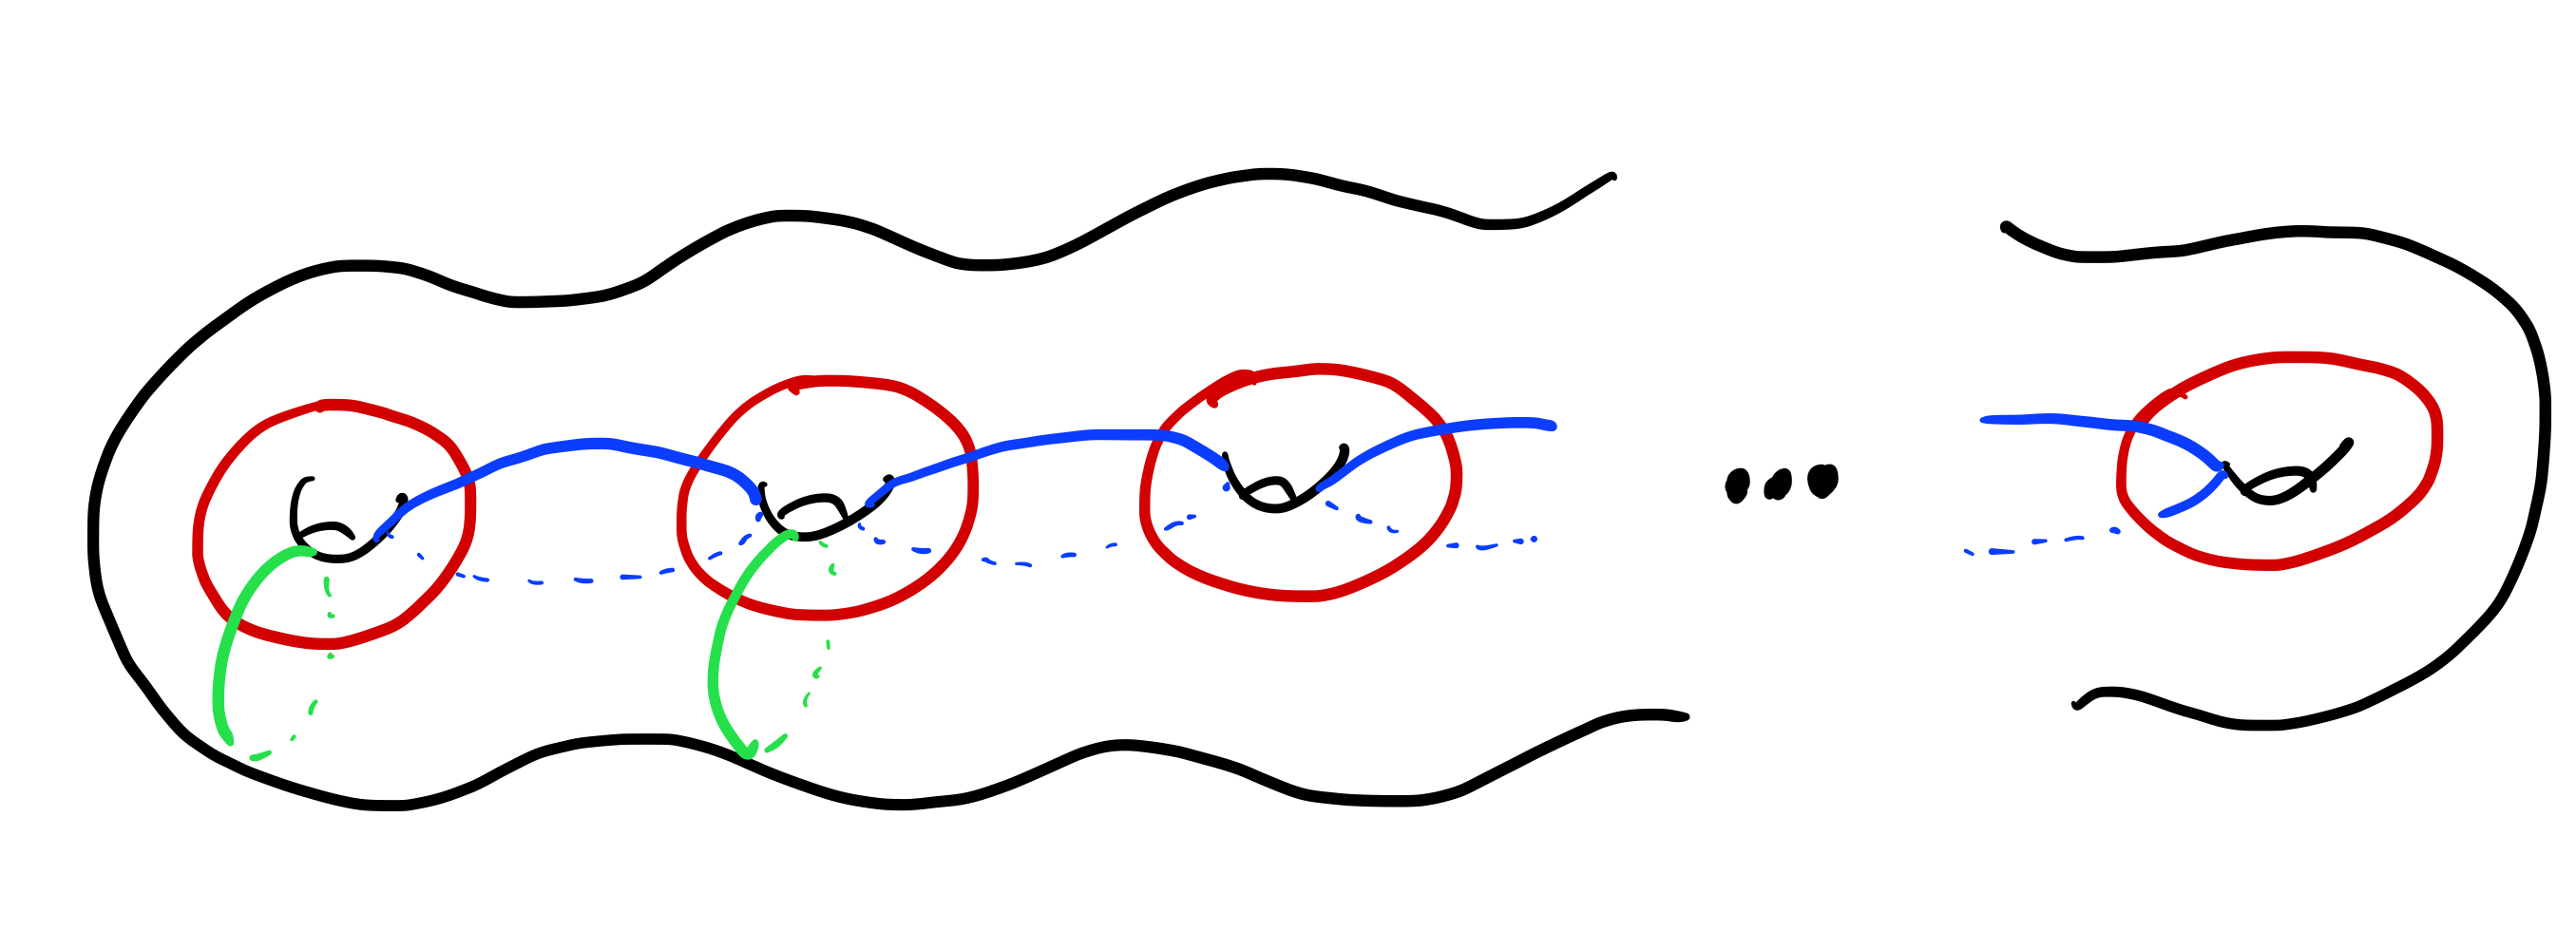
\includegraphics[width=0.9\linewidth]{fig0}
		\end{figure}
	\end{teo}
	\end{frame}
	
		\begin{frame}{Generadores de Humphries}
	Recordemos que los giros de Dehn actúan de la siguiente forma. Tomando como ejemplo una de las curvas verdes y una vecindad suya con una curva naranja de referencia,
	
	\begin{figure}[H]
		\centering
		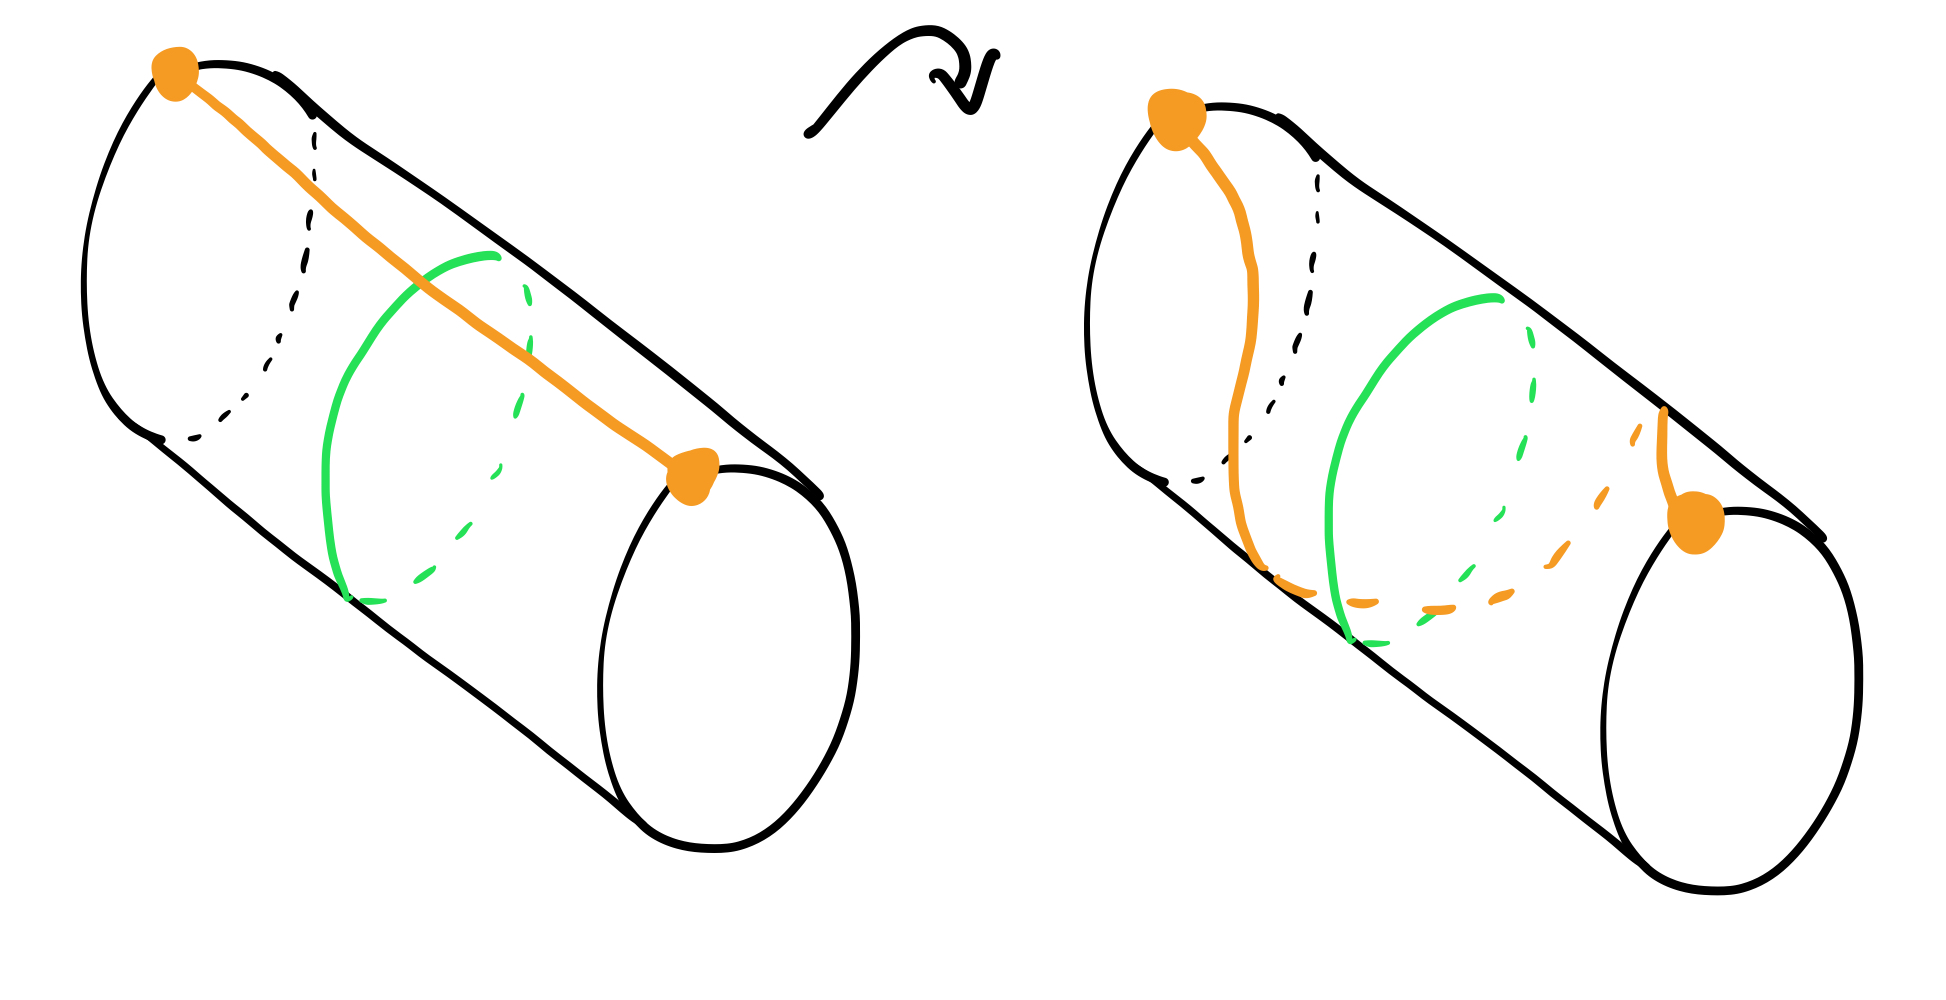
\includegraphics[width=0.7\linewidth]{fig0p}
	\end{figure}
	\end{frame}
	
	\section{Preliminares\\
		{\small Generadores de $\Mod(S_{0,n})$}}
		
	\begin{frame}{Generadores de $\Mod(S_{0,n})$}
		Para el caso de la esfera con puntos marcados, consideremos la siguiente sucesión exacta:
		\[\begin{tikzcd}[ampersand replacement=\&]
			1\arrow[r]\&\PMod(S_{0,n})\arrow[hook,r]\&\Mod(S_{0,n})\arrow[r,two heads]\&\Sigma_n\arrow[r]\&1
		\end{tikzcd}\]
		donde la flecha inyectiva es la inclusión y la suprayectiva es la acción de cada homeomorfismo de $S_{0,n}$ en la colección de puntos marcados vista como una permutación ($\Sigma_n$ es el grupo de permutaciones de $n$ elementos).
	\end{frame}
	
	\begin{frame}{Generadores de $\Mod(S_{0,n})$}
		\[\begin{tikzcd}[ampersand replacement=\&]
			1\arrow[r]\&\PMod(S_{0,n})\arrow[hook,r]\&\Mod(S_{0,n})\arrow[r,two heads]\&\Sigma_n\arrow[r]\&1
		\end{tikzcd}\]
Esta sucesión exacta implica que
\[\frac{\Mod(S_{0,n})}{\PMod(S_{0,n})}\approx\Sigma_n\]
Por lo tanto, este cociente está generado por los levantamientos de una colección de generadores de $\Sigma_n$. Es natural escoger las transposiciones para generar el grupo de permutaciones, que se levantan a mapping classes como mostramos a continuación.
	\end{frame}
	
		\begin{frame}{Generadores de $\Mod(S_{0,n})$}
		Tomemos el ejemplo de un disco con tres puntos marcados:
		\begin{figure}[H]
			\centering
			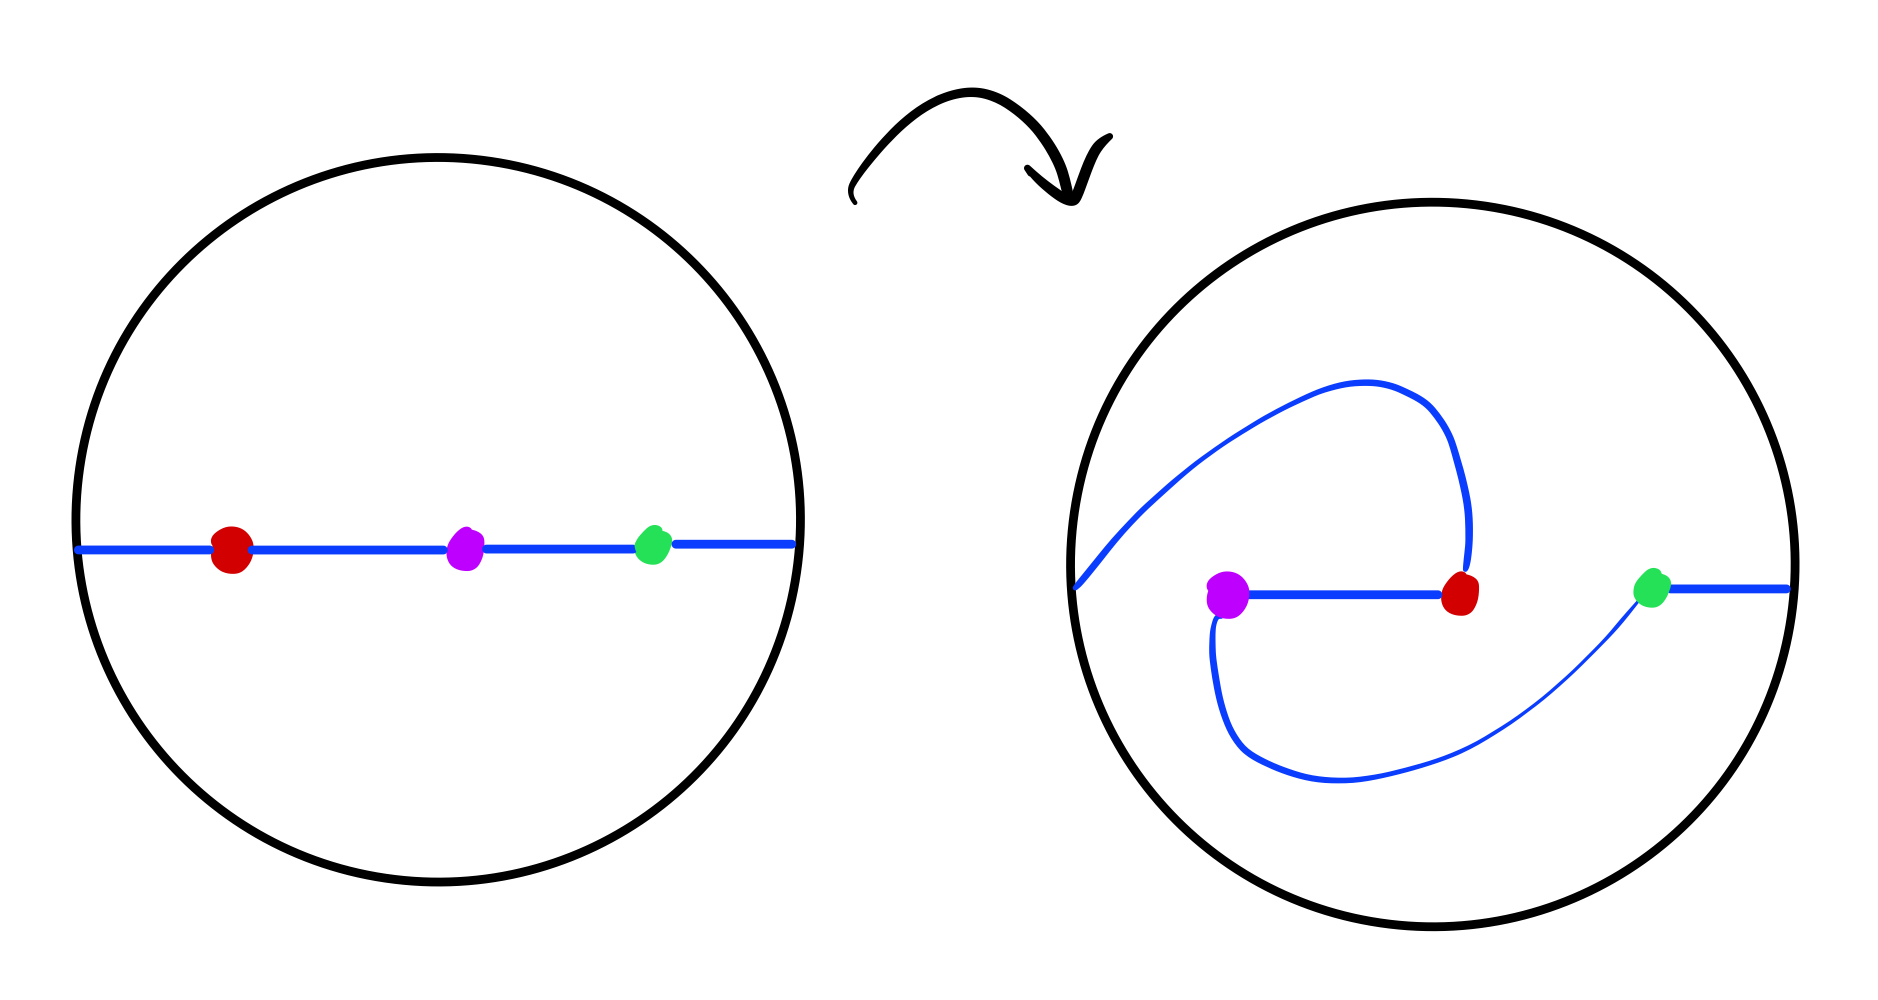
\includegraphics[width=.7\linewidth]{fig6}
		\end{figure}\vspace{-1cm}
		La permutación representada intercambia los puntos marcados rojo y morado. La curva azul nos sirve para visualizar la acción del homeomorfismo en todo el disco. Decimos que este homeomorfismo es un \textbf{\textit{medio giro}}.
	\end{frame}
	
		\begin{frame}{Generadores de $\Mod(S_{0,n})$}
		Como teníamos que
		\[\frac{\Mod(S_{0,n})}{\PMod(S_{0,n})}\approx\Sigma_n\]
		concluimos que $\Mod(S_{0,n})$ está generado por una colección de medios giros y una colección de generadores de $\PMod(S_{0,n})$. \pause De hecho,
		
		\begin{teo}
			Para $n\geq0$, el grupo $\PMod(S_{0,n})$ está generado por una cantidad finita de giros de Dehn.
		\end{teo}.
	\end{frame}
	
		\begin{frame}{Generadores de $\Mod(S_{0,n})$}
		\begin{teo}
			Para $n\geq0$, el grupo $\PMod(S_{0,n})$ está generado por una cantidad finita de giros de Dehn.
		\end{teo}
		
		Este resultado es la restricción de la \textbf{\textit{sucesión exacta de Birman}} a $\Mod(S_{n,g})$):
		\textcolor{blue}{
		\[\begin{tikzcd}[ampersand replacement=\&,column sep=small]
			1\arrow[r]\&\pi_1(S_{g,n})\arrow[r]\&\PMod(S_{g,n+1})\arrow[r]\&\PMod(S_{g,n})\arrow[r]\&1
		\end{tikzcd}\]}
		Iterando esta sucesión partiendo de que $\PMod(S_{0,n})=1$ para $n\leq3$ y conociendo los grupos fundamentales de cada esfera con puntos marcados, se concluye que $\PMod(S_{0,n})$ es una extensión iterada de grupos libres. \pause Por ejemplo, $\PMod(S_{0,4})\approx F_2$ y $\PMod(S_{0,5})\approx F_2\ltimes F_3$.
	\end{frame}
	
			\begin{frame}{Generadores de $\Mod(S_{0,n})$}
%		\begin{teo}
%			Para $n\geq0$, el grupo $\PMod(S_{0,n})$ está generado por una cantidad finita de giros de Dehn.
%		\end{teo}
%		
				Por ejemplo, $\PMod(S_{0,4})\approx F_2$ y $\PMod(S_{0,5})\approx F_2\ltimes F_3$.
	\textcolor{blue}{
		\[\begin{tikzcd}[ampersand replacement=\&,column sep=small]
			1\arrow[r]\&\pi_1(S_{g,n})\arrow[r]\&\PMod(S_{g,n+1})\arrow[r]\&\PMod(S_{g,n})\arrow[r]\&1
		\end{tikzcd}\]}
		\pause Recordemos que si la sucesión exacta
		\[\begin{tikzcd}[ampersand replacement=\&]
			1\arrow[r]\&K\arrow[r]\&G\arrow[r]\&Q\arrow[r]\&1
		\end{tikzcd}\]
		se \textbf{\textit{escinde}}, $G\approx Q\ltimes K$. En estos casos, la sucesión se escinde porque el grupo de la derecha es libre. (La sucesión exacta de Birman no siempre se escinde).
	\end{frame}
	
	\begin{frame}{Generadores de $\Mod(S_{0,n})$}
Finalmente observemos cómo funciona la flecha que sale del grupo fundamental:
			\textcolor{blue}{
			\[\begin{tikzcd}[ampersand replacement=\&,column sep=small]
				1\arrow[r]\&\pi_1(S_{g,n})\arrow[r]\&\PMod(S_{g,n+1})\arrow[r]\&\PMod(S_{g,n})\arrow[r]\&1
			\end{tikzcd}\]}
		\pause A un representante de $[\alpha]\in\pi_1(S_{g,n})$ le asociamos dos curvas $a$ y $b$ que están un poco a la izquierda y a la derecha de $\alpha$.
		\begin{figure}[H]
			\centering
			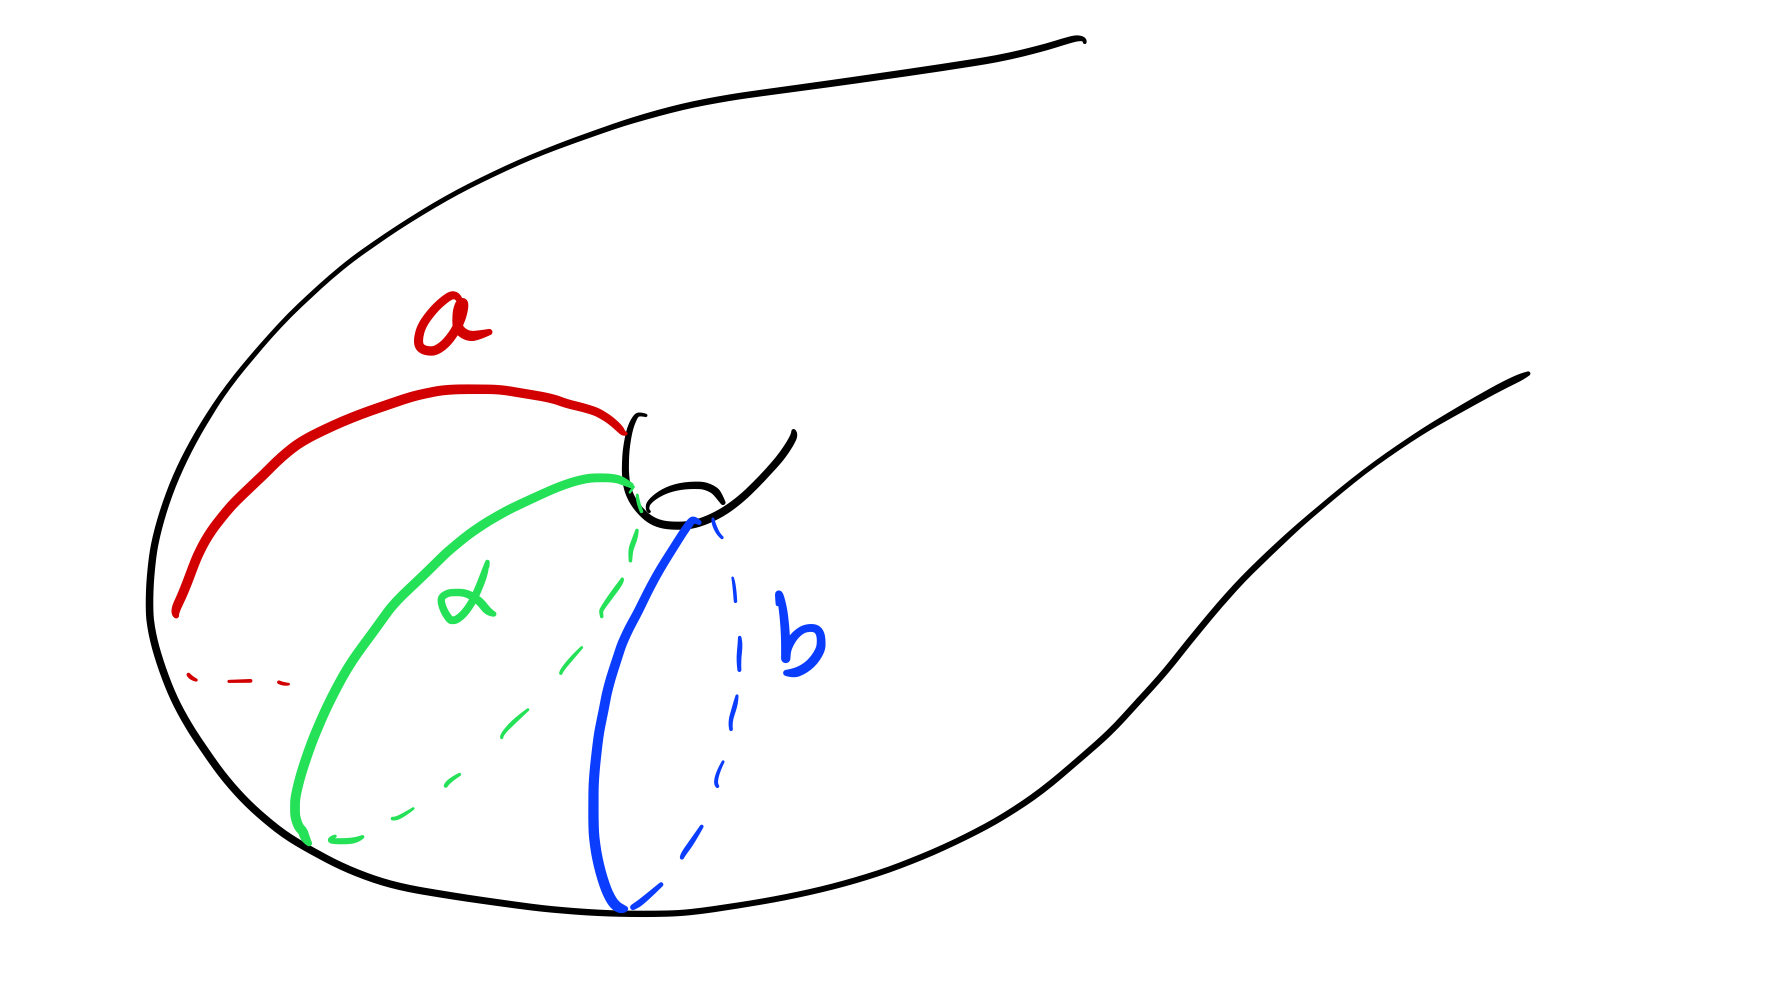
\includegraphics[width=.5\linewidth]{fig20}
		\end{figure}
	\end{frame}
	
		\begin{frame}{Generadores de $\Mod(S_{0,n})$}
		\textcolor{blue}{
			\[\begin{tikzcd}[ampersand replacement=\&,column sep=small]
				1\arrow[r]\&\pi_1(S_{g,n})\arrow[r,"\mathcal{P}"]\&\PMod(S_{g,n+1})\arrow[r]\&\PMod(S_{g,n})\arrow[r]\&1
			\end{tikzcd}\]}
		A un representante de $[\alpha]\in\pi_1(S_{g,n})$ le asociamos dos curvas $a$ y $b$ que están un poco a la izquierda y a la derecha de $\alpha$.
		\begin{figure}[H]
			\centering
			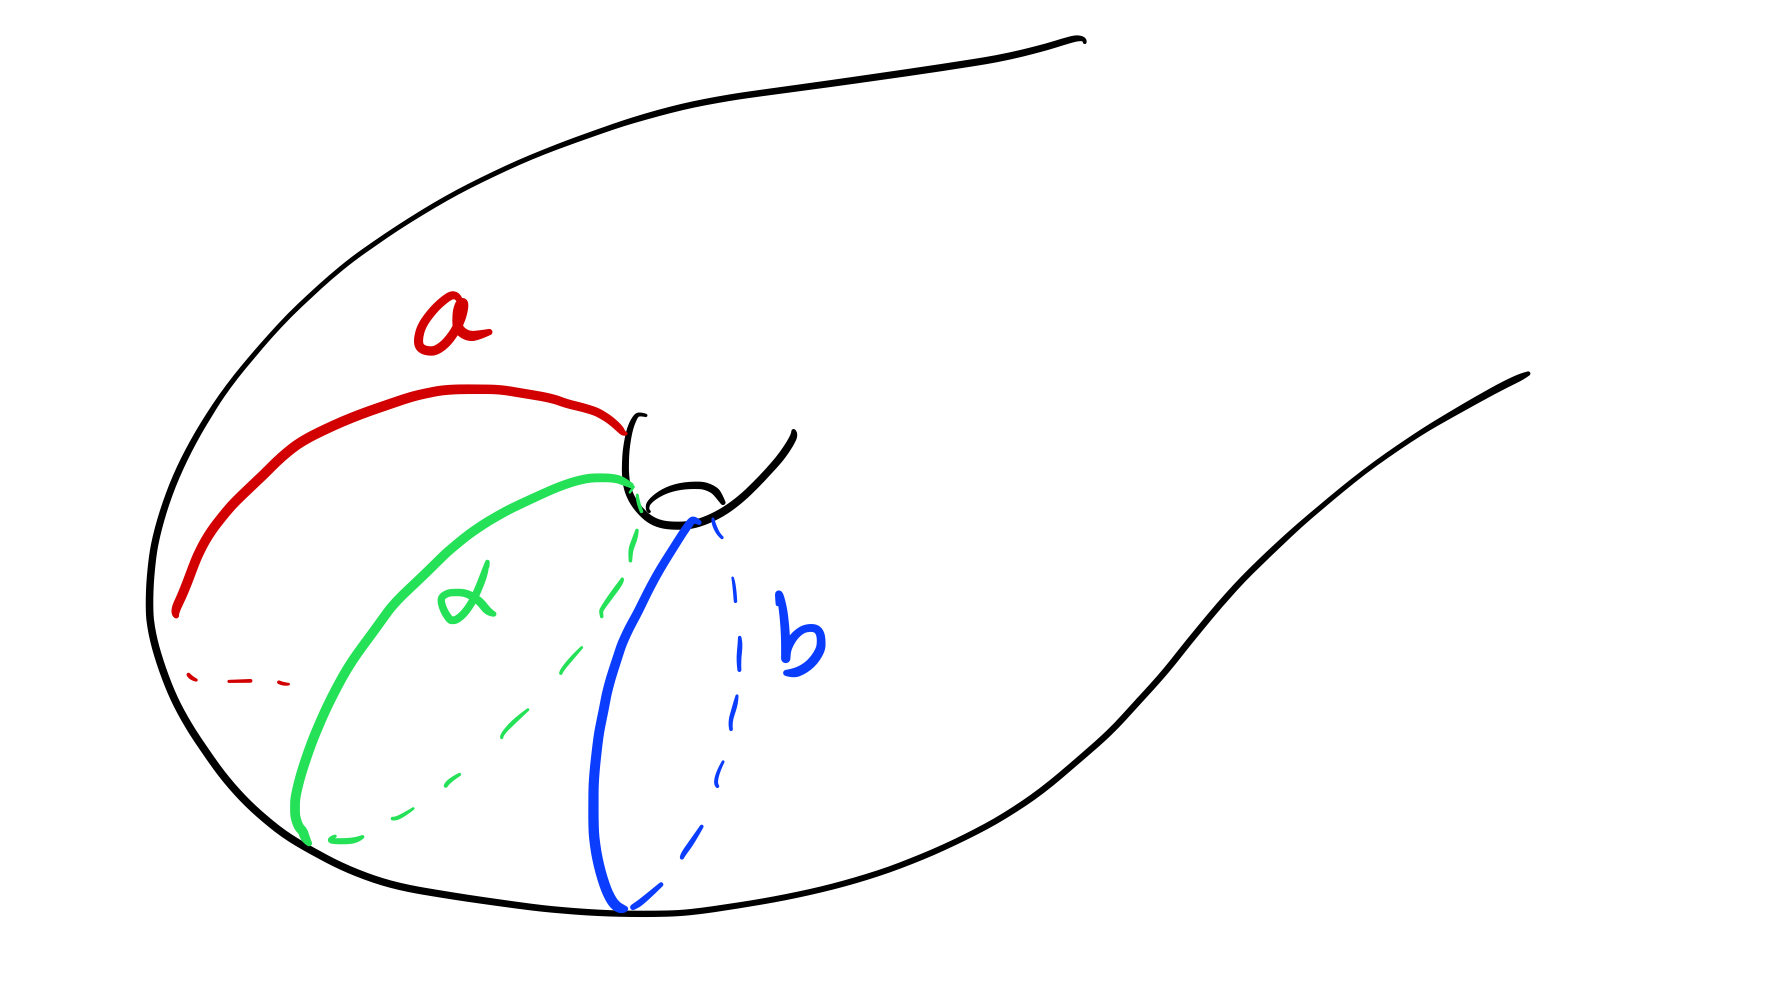
\includegraphics[width=.5\linewidth]{fig20}
		\end{figure}
		 Si $T_a$ y $T_b$ son los giros de Dehn respecto a $a$ y $b$,
		\[\alpha\xmapsto{\mathcal{P}ush}T_aT_b^{-1}\]
	\end{frame}
	
	\begin{frame}{Generadores de $\Mod(S_{0,n})$}
	En conclusión,
	
	\begin{itemize}
		\item $\PMod(S_{0,n})$ es una extensión de grupos libres cuyos generadores son productos de giros de Dehn, y esto implica que
		
		\item $\Mod(S_{0,n})$ está generado por esos productos de giros de Dehn y una colección de medios giros.
	\end{itemize}
	\end{frame}
	

\section{Una presentación de $\Mod(S_2)$}
\begin{frame}

\begin{itemize}
	\item Para encontrar una presentación de $\Mod(S_2)$ usaremos el isomorfismo $\SMod(S)/D\cong\LMod(X)$\pause
	\item Sabemos que la involución hiperelíptica $\iota$ induce un cubriente \[\iota:S_g\to S^2_{0,2g+2}\]
	es decir, de la superficie de género $g$ en la esfera con $2g+2$ puntos marcados. \pause 

	\item El grupo de transformaciones de deck es $\langle \iota\rangle$, que es soluble.\pause
	
	\item Como $S_2$ es una superficie hiperbólica, por el teorema de Birman-Hilden y sus equivalencias tenemos que
	\[\SMod(S_g)/\langle\iota\rangle\cong\LMod(S_{0,2g+2})\]
\end{itemize}
\end{frame}

\begin{frame}{$\SMod(S_2)=\Mod(S_2)$}
	Para el caso de género 2, resulta ser que
	\[\SMod(S_2)=\Mod(S_2),\]
	es decir, cualquier mapping class de $S_2$ es simétrica respecto a la involución hiperelíptica.
\end{frame}

\begin{frame}{$\SMod(S_2)=\Mod(S_2)$}
Para verlo usamos los generadores de Humphries de $\Mod(S_2)$ que son los giros de Dehn respecto a las siguientes cinco curvas:
\begin{figure}[H]
	\centering
	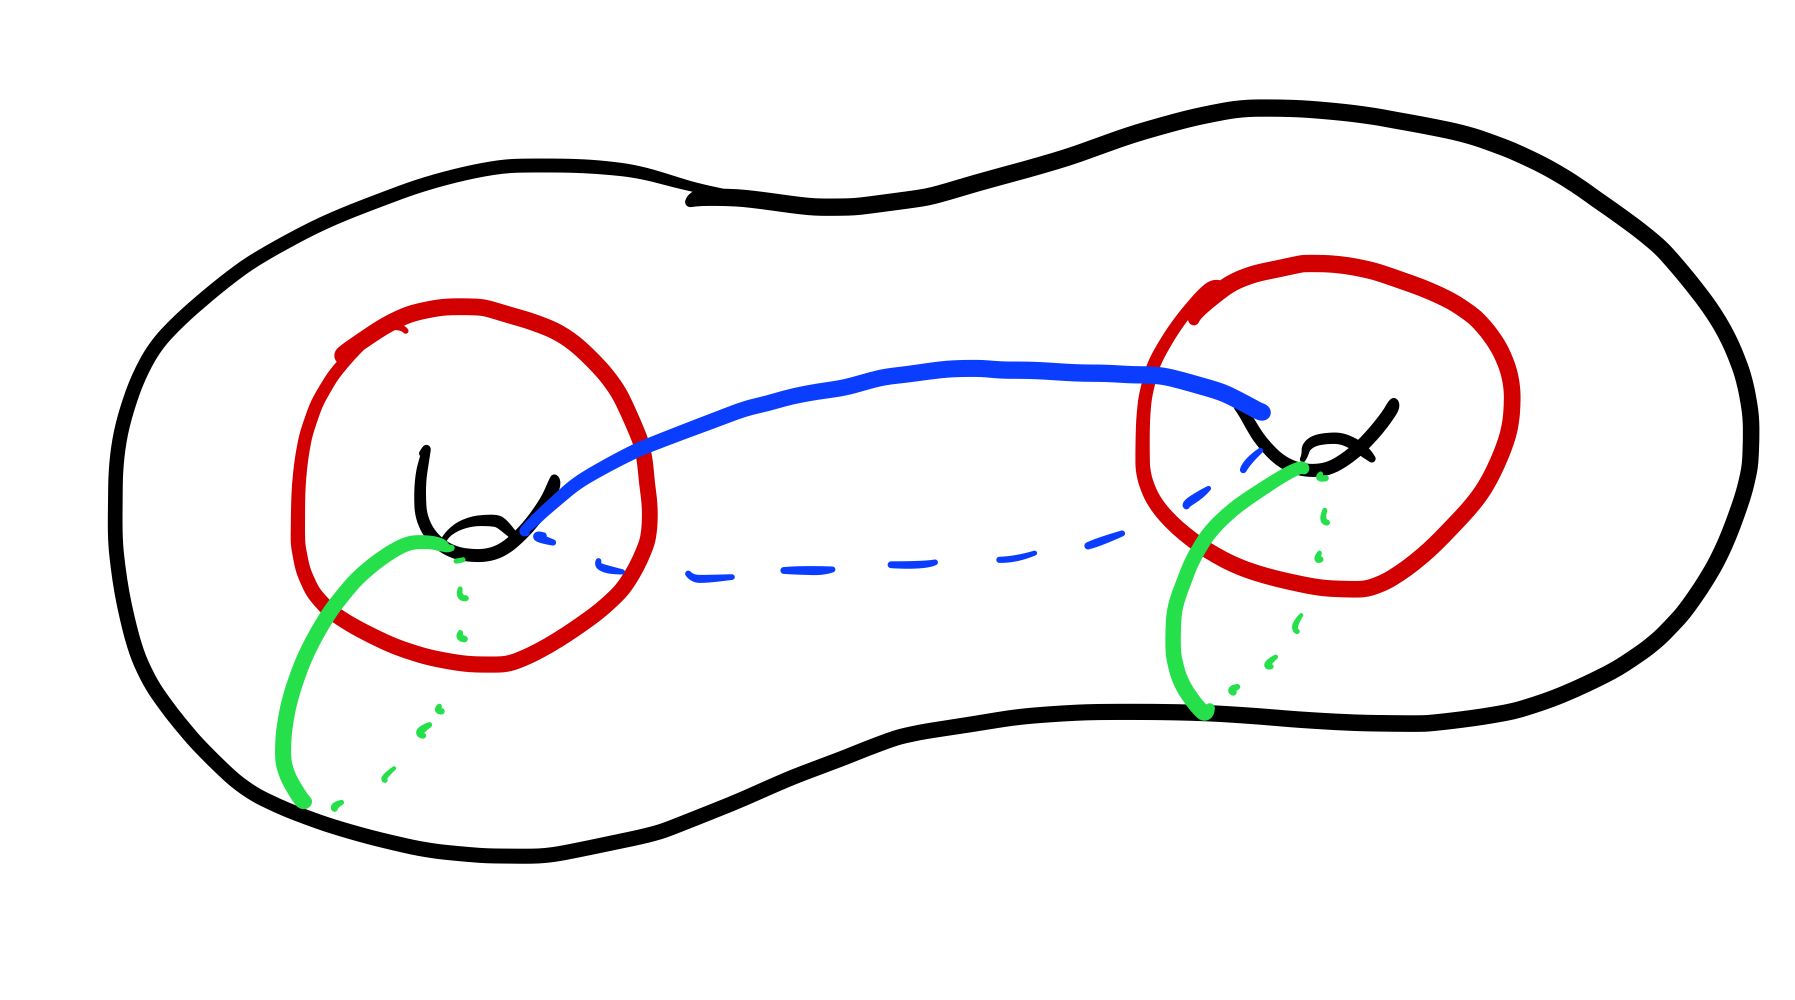
\includegraphics[width=0.7\linewidth]{fig1}
\end{figure}
\end{frame}


\begin{frame}{$\SMod(S_2)=\Mod(S_2)$}
Reacomodando ligeramente las curvas verde y azul, observamos que de hecho la involución hiperelíptica las fija:
\begin{figure}[H]
	\centering
	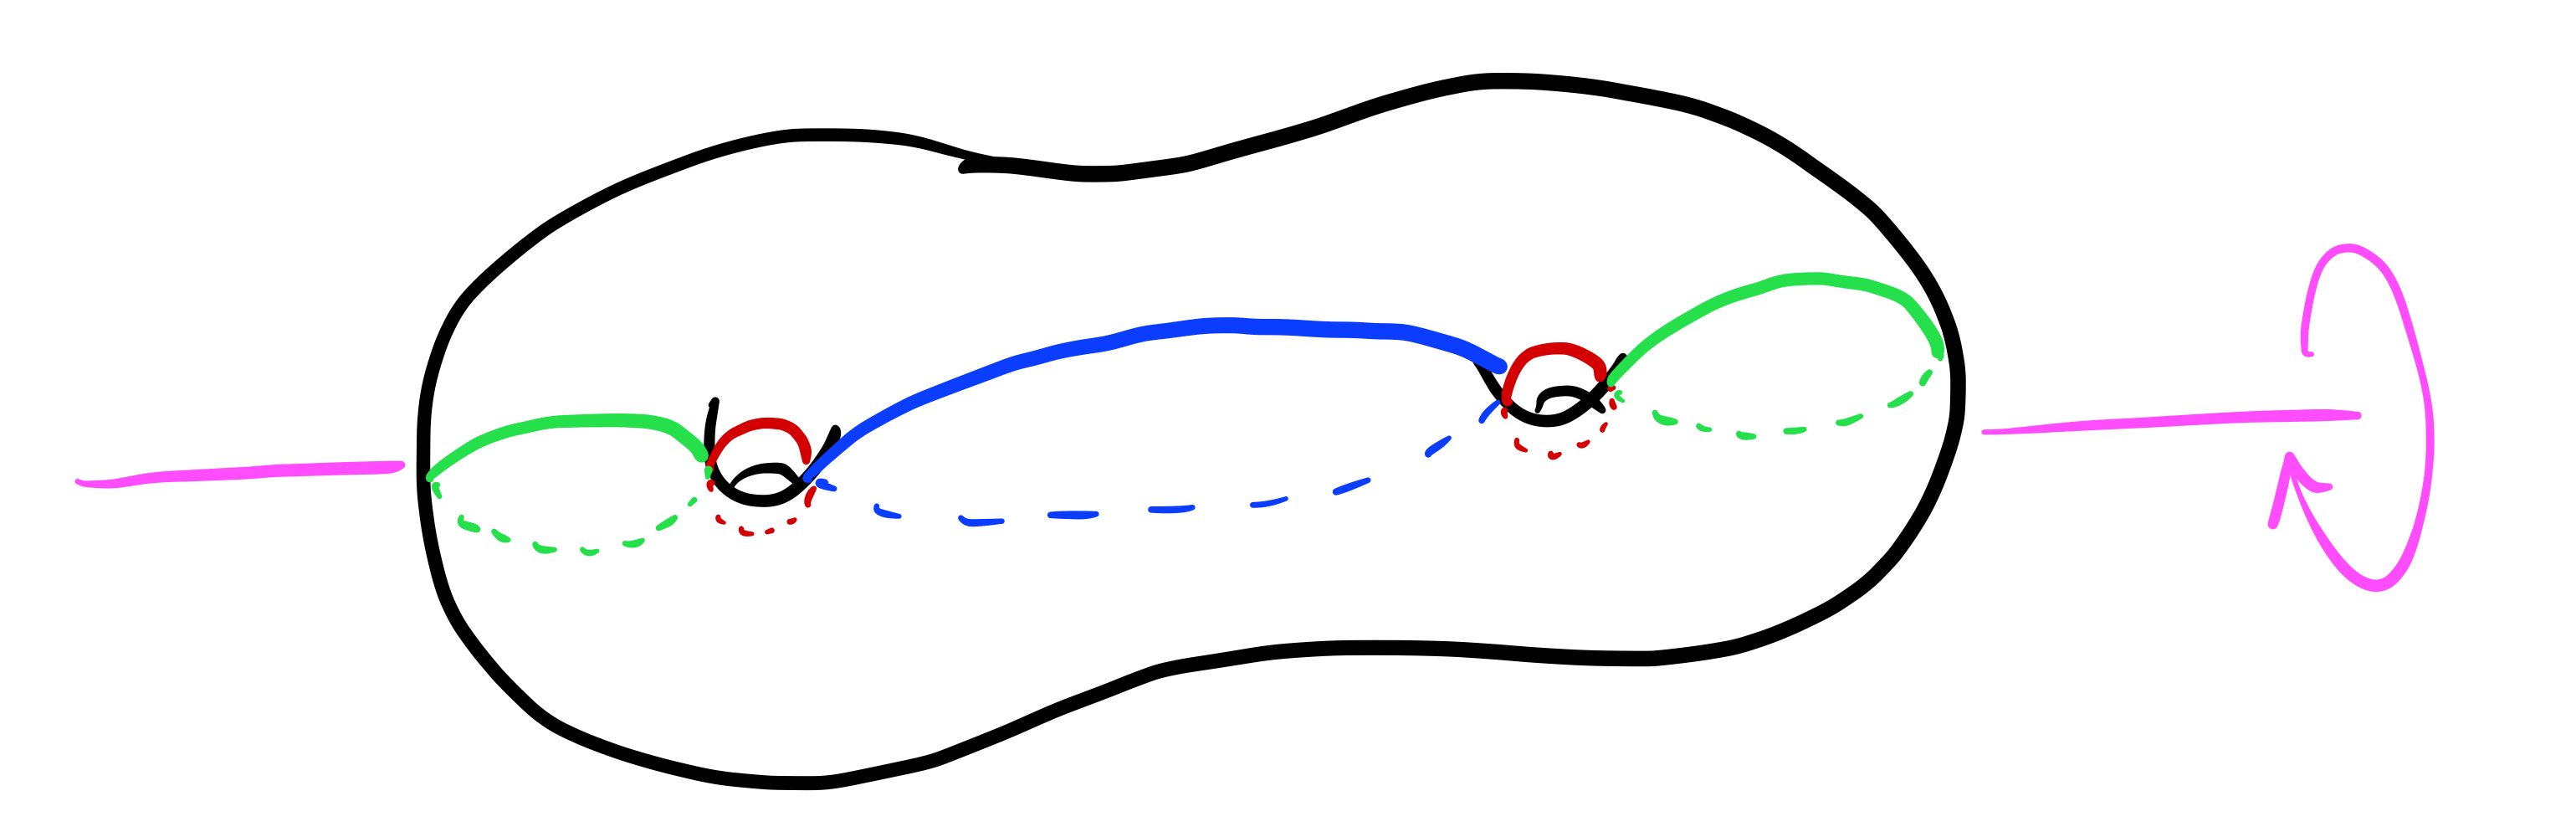
\includegraphics[width=\linewidth]{fig2}
\end{figure}
\pause De aquí se sigue que estos giros de Dehn mandan fibras en fibras. Veamos por qué.
\end{frame}

\begin{frame}{$\SMod(S_2)=\Mod(S_2)$}
	Tomemos el ejemplo del giro de Dehn respecto a una de las curvas verdes. Mostrando dos curvas de referencia morada y naranja, este giro actúa así:
	\begin{figure}[H]
		\centering
		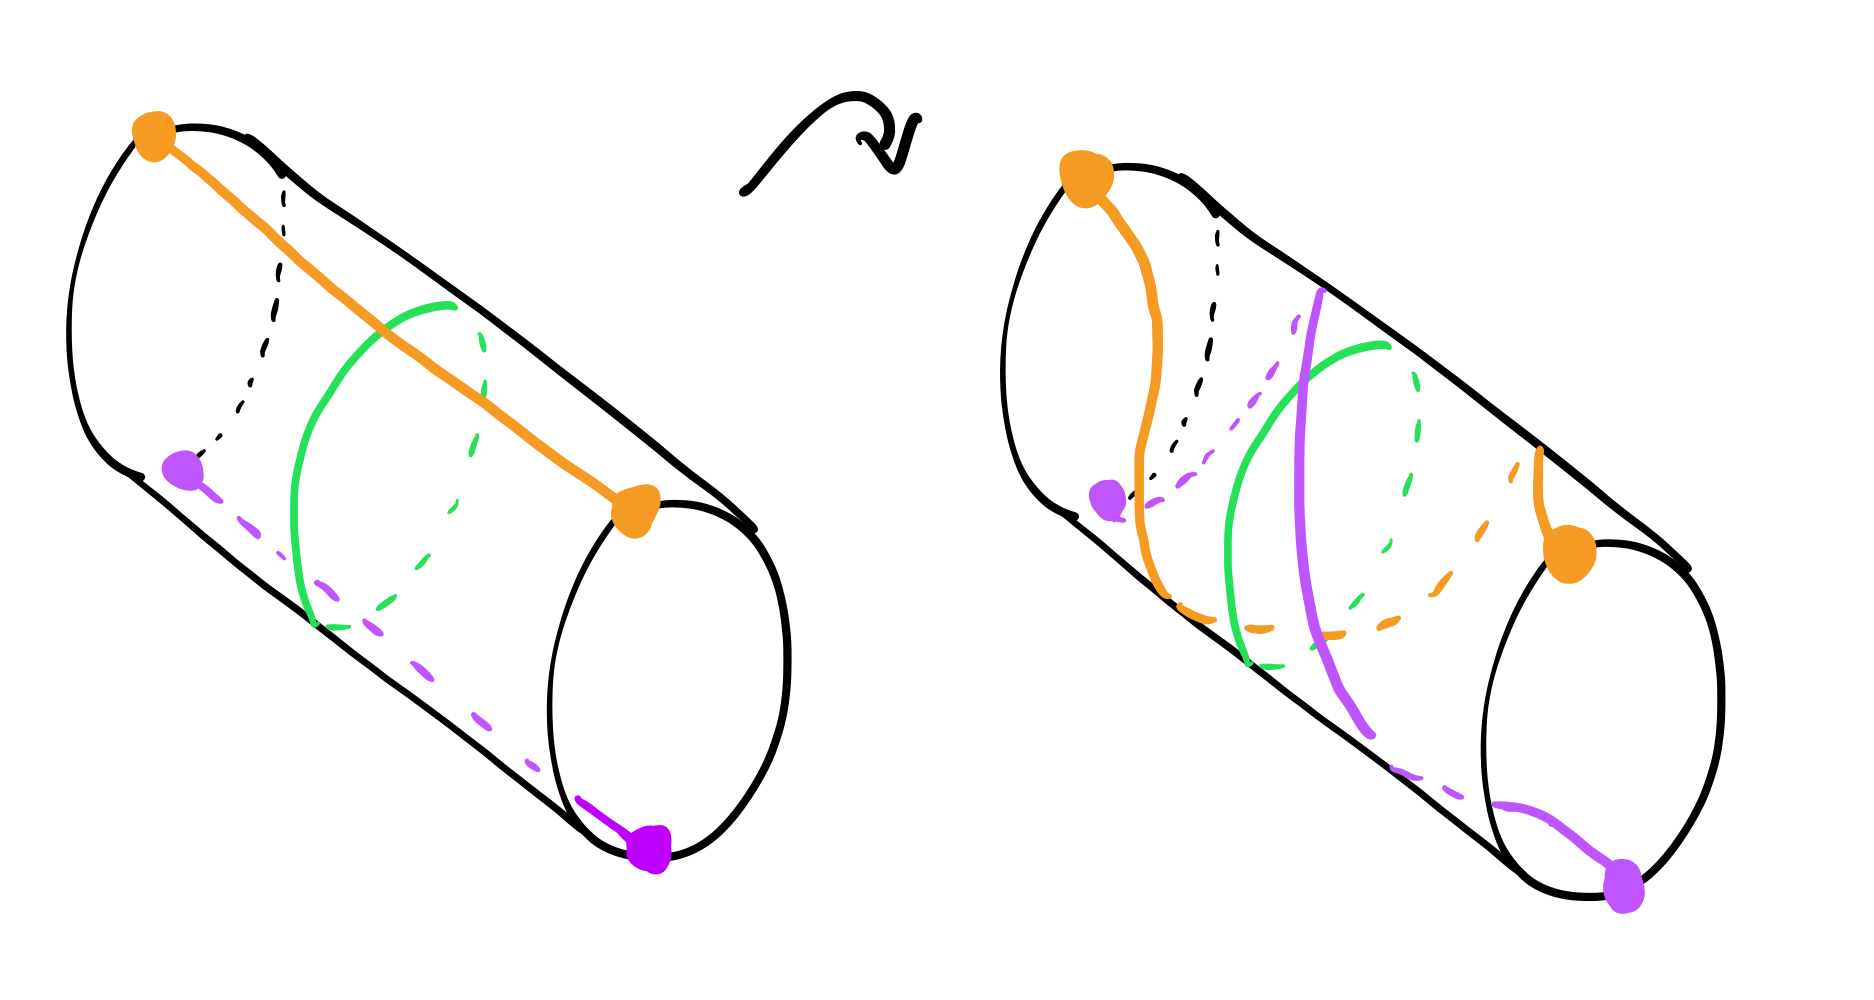
\includegraphics[width=.8\linewidth]{fig3}
	\end{figure}
\end{frame}

\begin{frame}{$\SMod(S_2)=\Mod(S_2)$}
	Ahora tomemos la fibra de algún punto en el cociente, es decir, dos puntos que se identifican mediante la involución hiperéliptica. Suponiendo que la curva azul y la verde están a la altura máxima y mínima de $S_2$, respectivamente, una fibra se ve así:
	
	\begin{figure}[H]
		\centering
		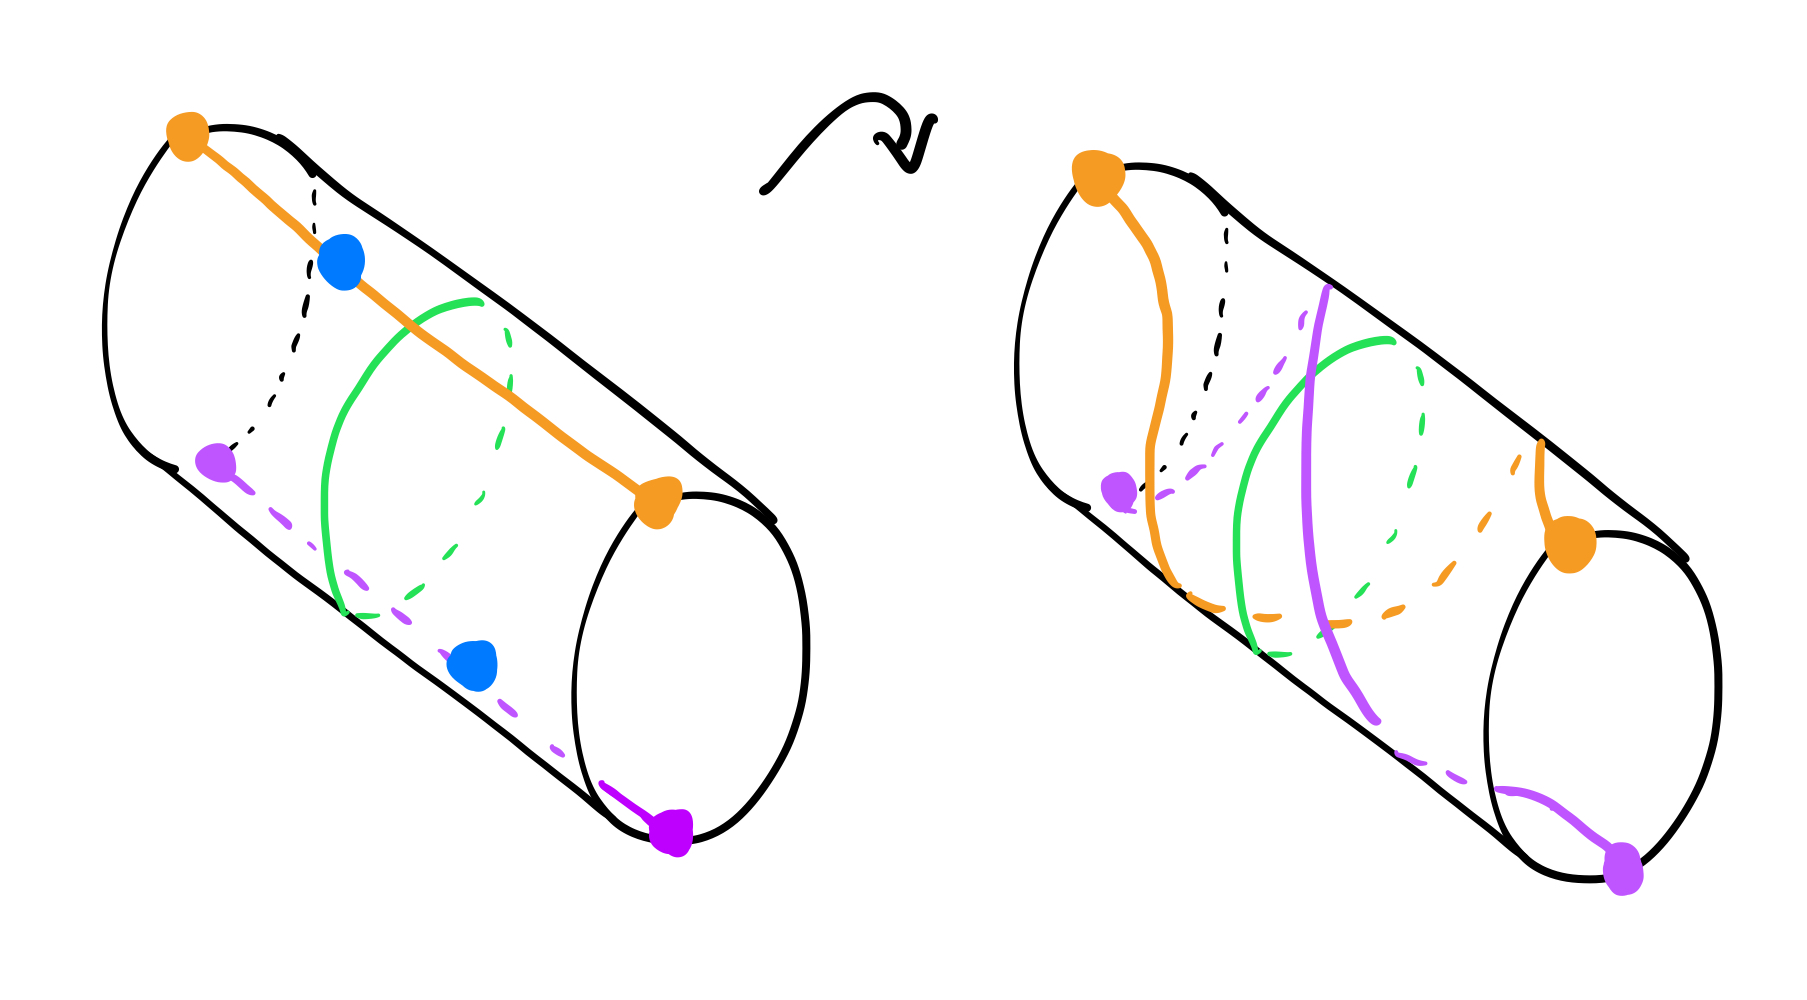
\includegraphics[width=.8\linewidth]{fig3.5}
	\end{figure}
\end{frame}

\begin{frame}{$\SMod(S_2)=\Mod(S_2)$}
	Y su imagen bajo el giro de Dehn se ve así:
	
	\begin{figure}[H]
		\centering
		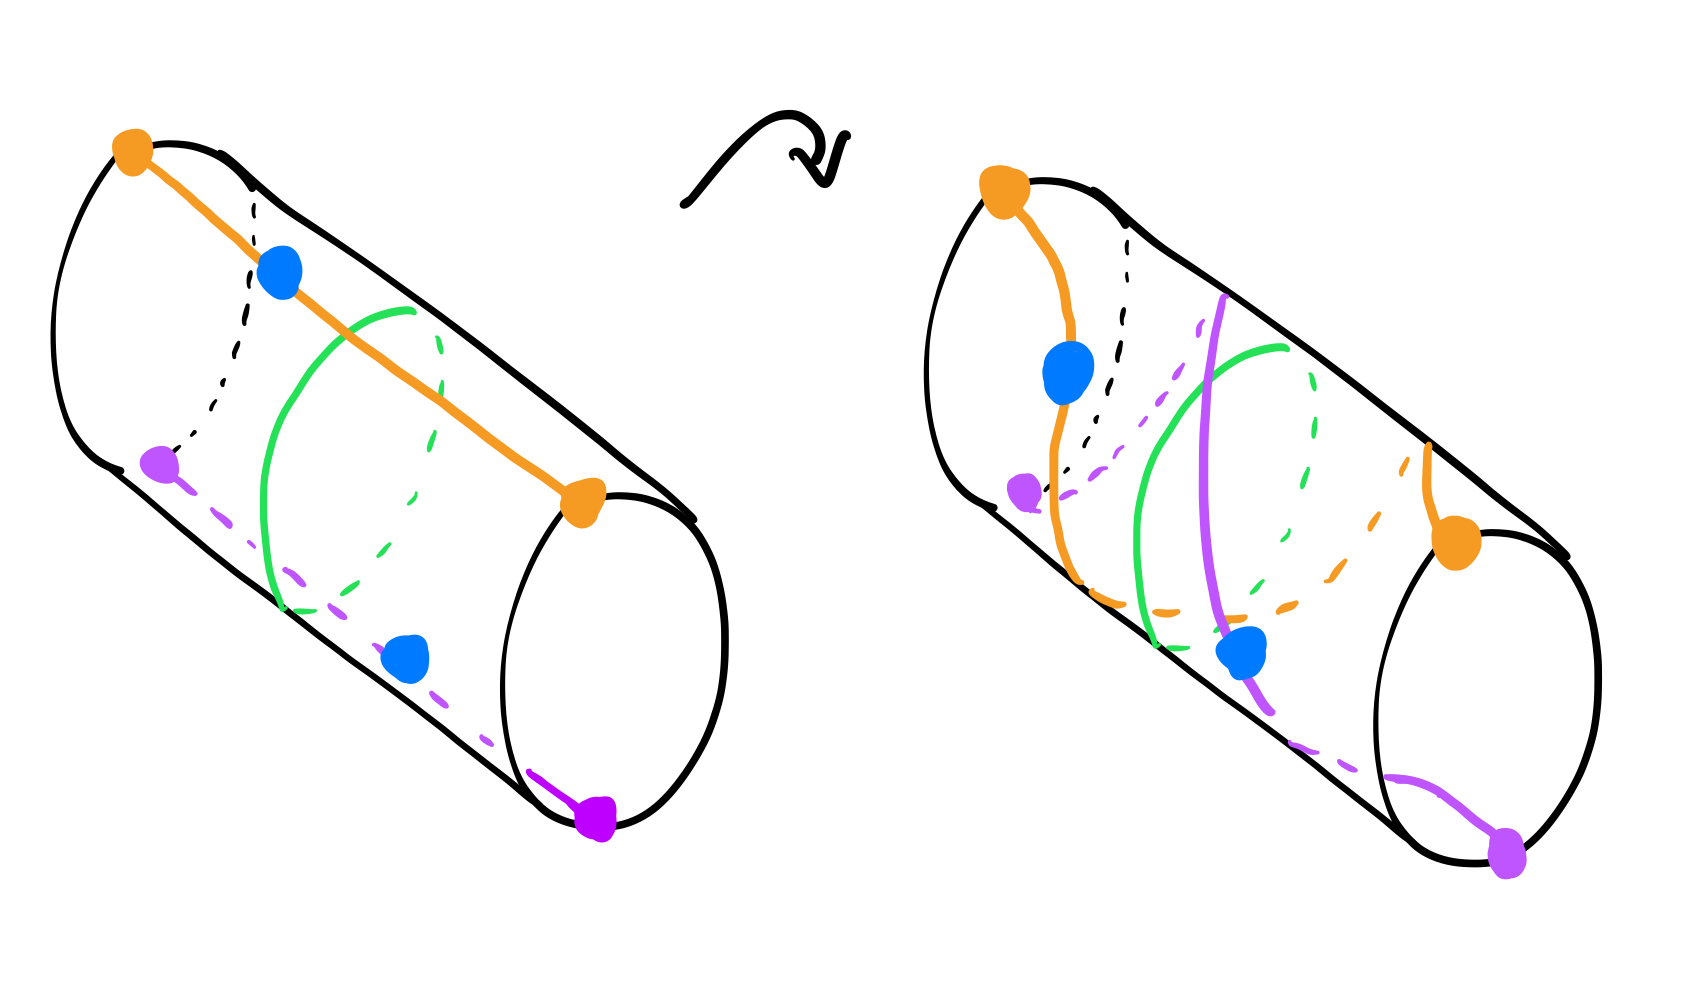
\includegraphics[width=.8\linewidth]{fig4}
	\end{figure}
		\pause ¿Realmente la pareja de puntos en la figura de la derecha es una fibra?
\end{frame}


\begin{frame}{$\SMod(S_2)=\Mod(S_2)$}

	
	\begin{figure}[H]
		\centering
		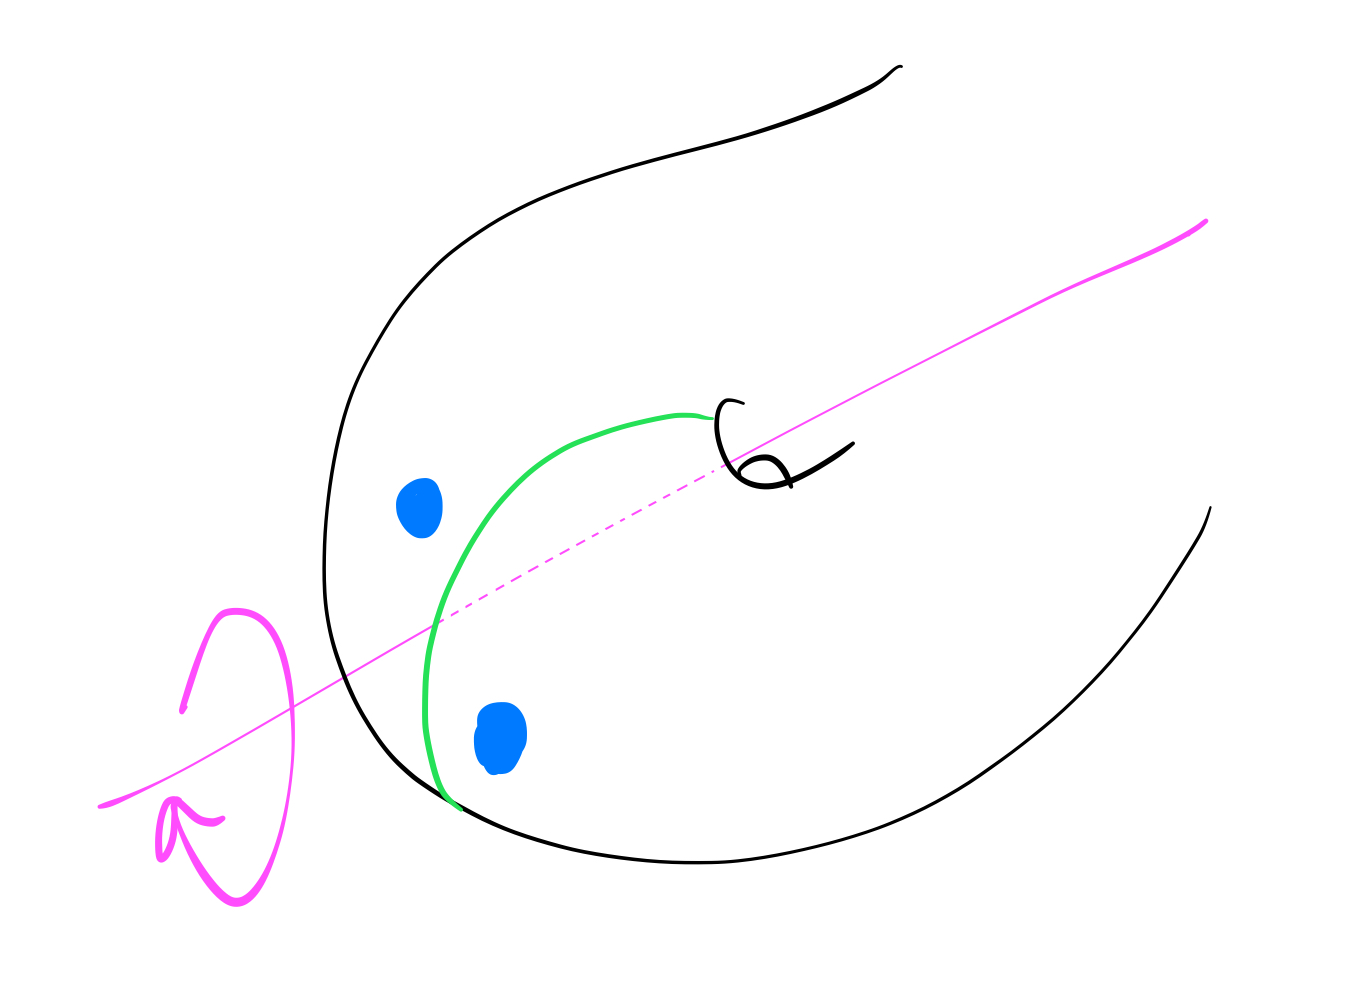
\includegraphics[width=.7\linewidth]{fig5}
	\end{figure}
	\begin{center}
		¡Sí!
	\end{center}
\end{frame}

\begin{frame}{$\SMod(S_2)=\Mod(S_2)$}
	Esto implica que
	\[\Mod(S_2)/\langle\iota\rangle\cong\LMod(S_{0,6}).\]
	\pause Ahora veamos qué pasas con el grupo del lado derecho.
\end{frame}

\begin{frame}{$\LMod(S_{0,6})\cong\Mod(S_{0,6})$}
	Resulta que
	\[\LMod(S_{0,6})\cong\Mod(S_{0,6})\]
	\pause Para verlo, recordemos que $\Mod(S_{0,6})$ está generado por una colección de productos de generadores de $\PMod(S_{0,6})$ y una colección de medios giros. \pause
	
	Primero veamos qué pasa con los generadores de $\PMod(S_{0,6})$. \pause Recordemos que son productos de giros de Dehn respecto a parejas de curvas alrededor de elementos en $\pi_1(S_{0,6})$.
\end{frame}

\begin{frame}{$\LMod(S_{0,6})\cong\Mod(S_{0,6})$}
		\begin{figure}[H]
		\centering
		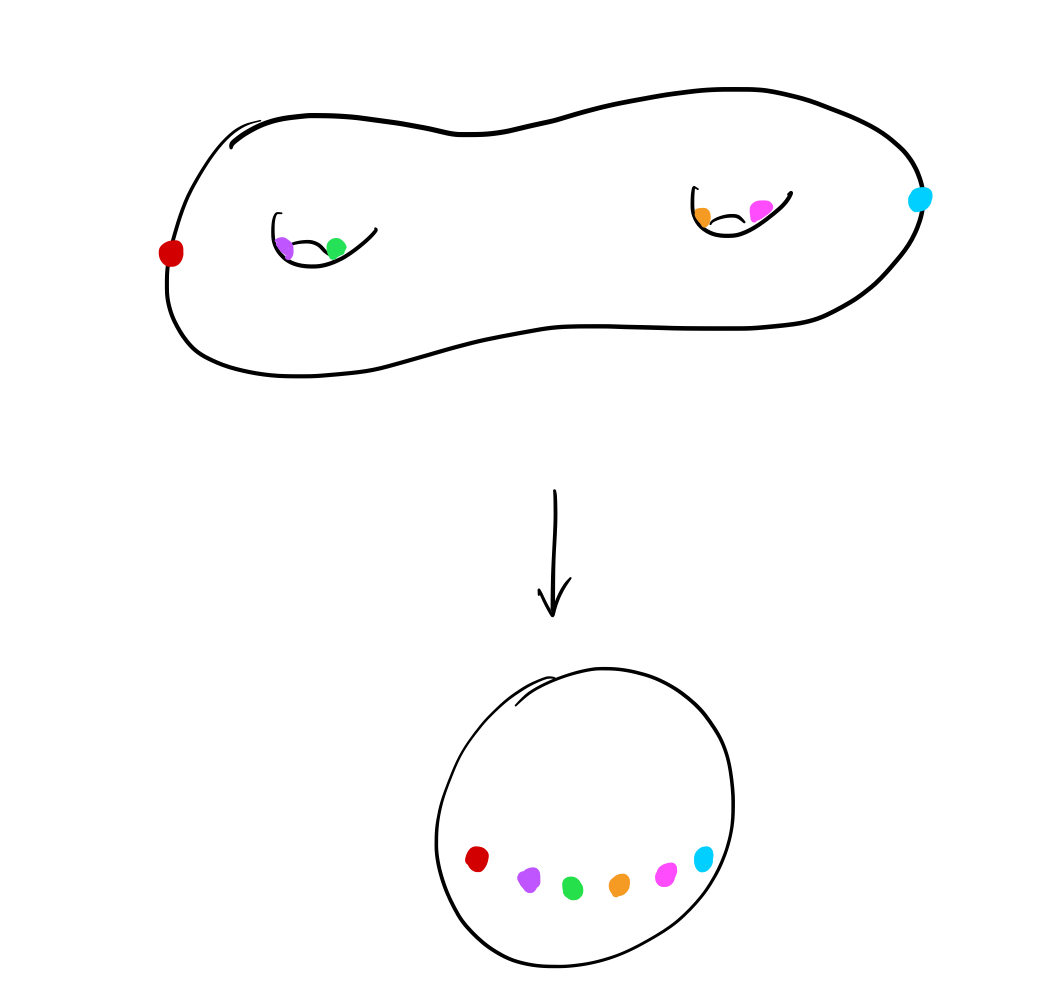
\includegraphics[width=.5\linewidth]{fig21}
	\end{figure}
\end{frame}

\begin{frame}{$\LMod(S_{0,6})\cong\Mod(S_{0,6})$}
	\begin{figure}[H]
		\centering
		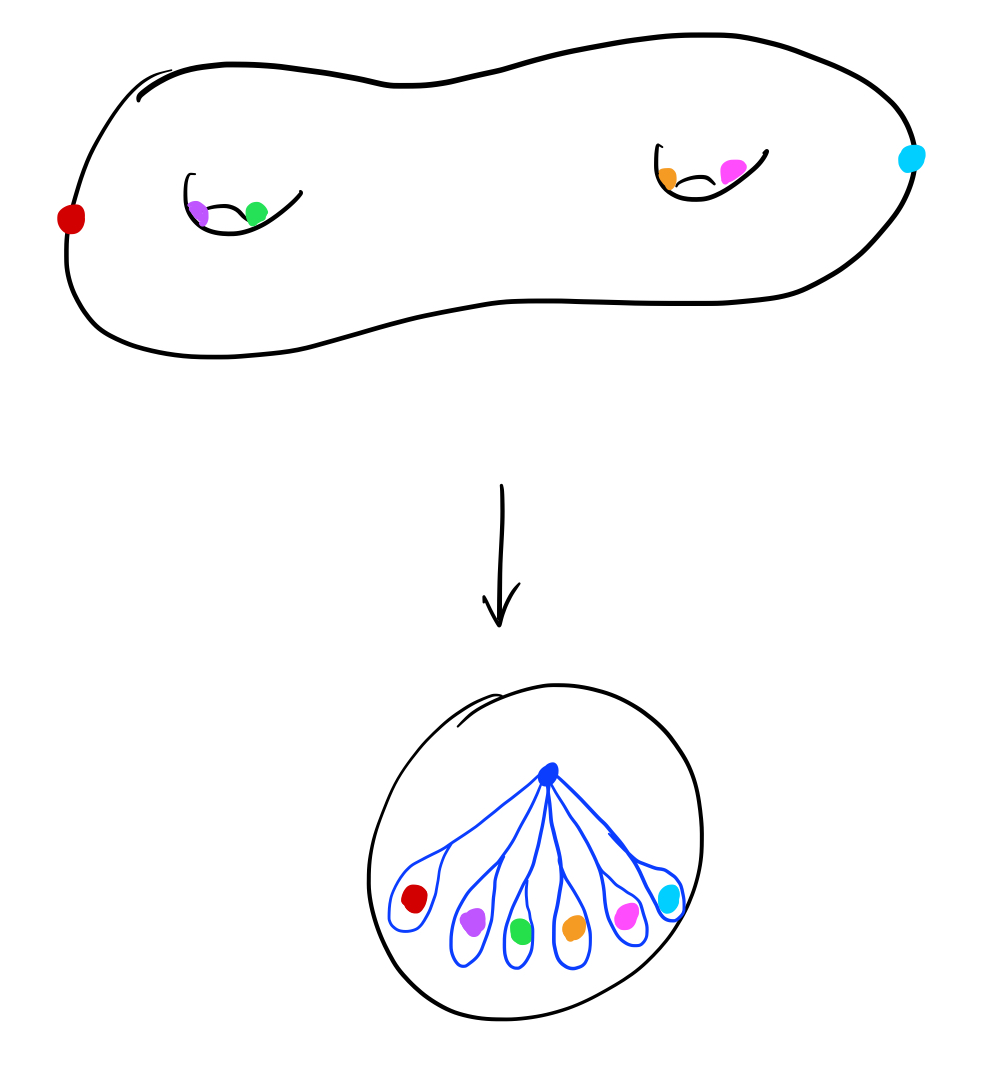
\includegraphics[width=.5\linewidth]{fig22}
	\end{figure}
\end{frame}

\begin{frame}{$\LMod(S_{0,6})\cong\Mod(S_{0,6})$}
	\begin{figure}[H]
		\centering
		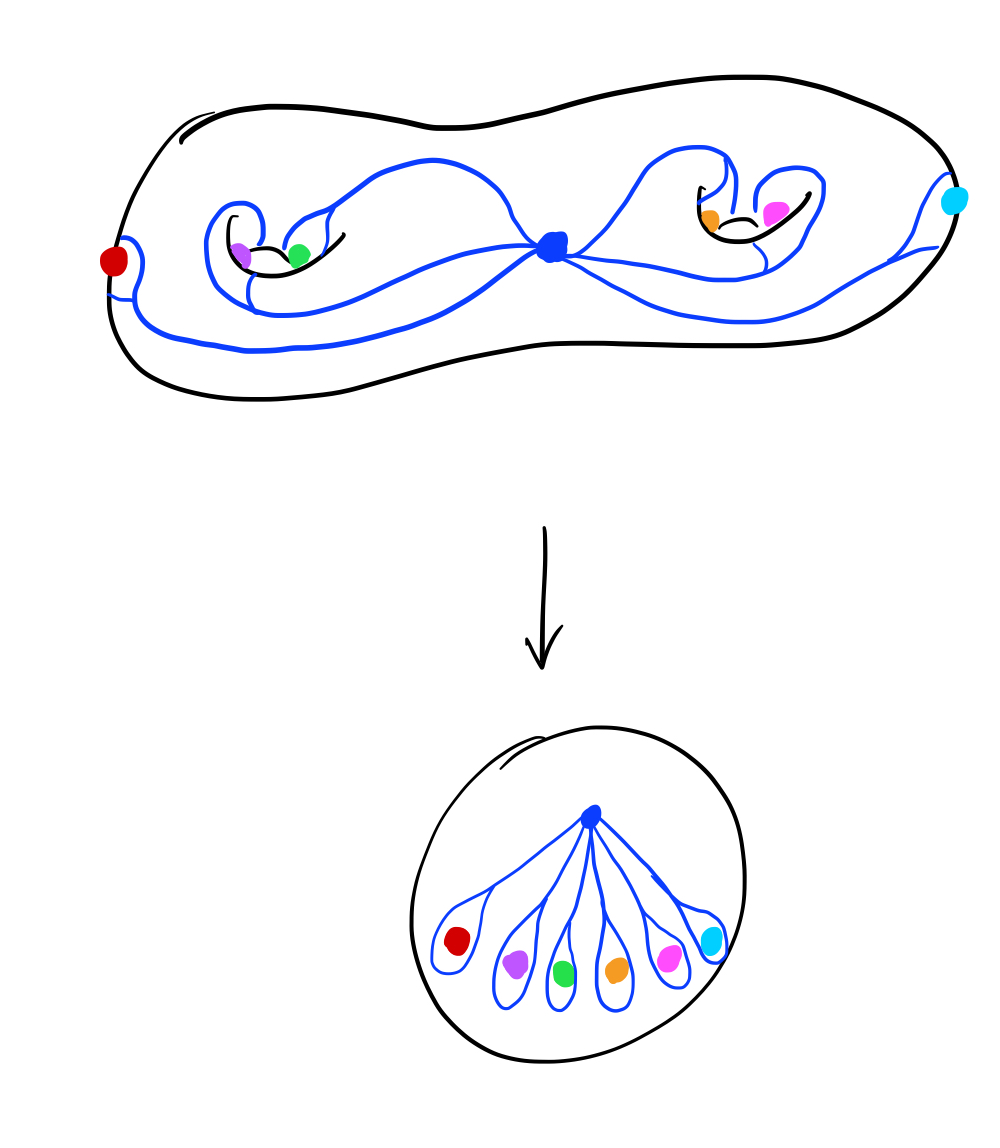
\includegraphics[width=.5\linewidth]{fig23}
	\end{figure}
		\begin{center}
		¡Los levantamientos son curvas contraibles!
	\end{center}
\end{frame}

\begin{frame}{$\LMod(S_{0,6})\cong\Mod(S_{0,6})$}
	Ahora veamos qué pasa con los medios giros en nuestro cubriente.\pause
	\begin{figure}[H]
		\centering
		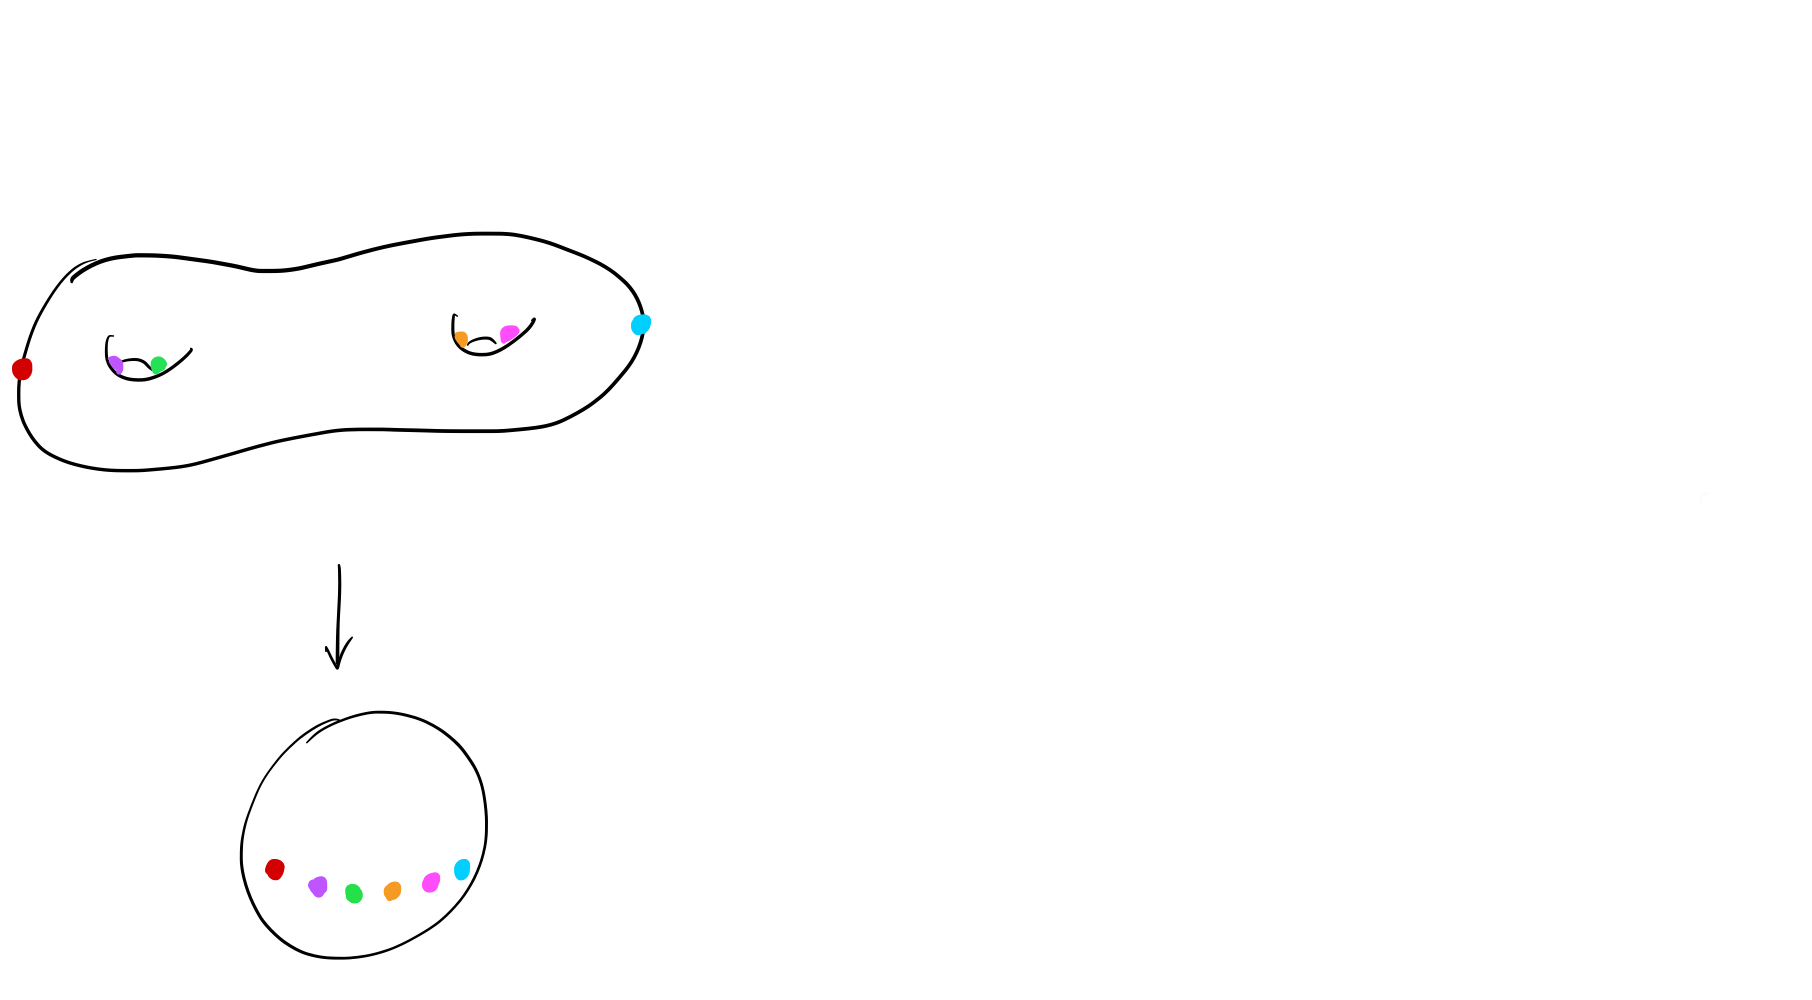
\includegraphics[width=1\linewidth]{fig24}
	\end{figure}
\end{frame}

\begin{frame}{$\LMod(S_{0,6})\cong\Mod(S_{0,6})$}

	\begin{figure}[H]
		\centering
		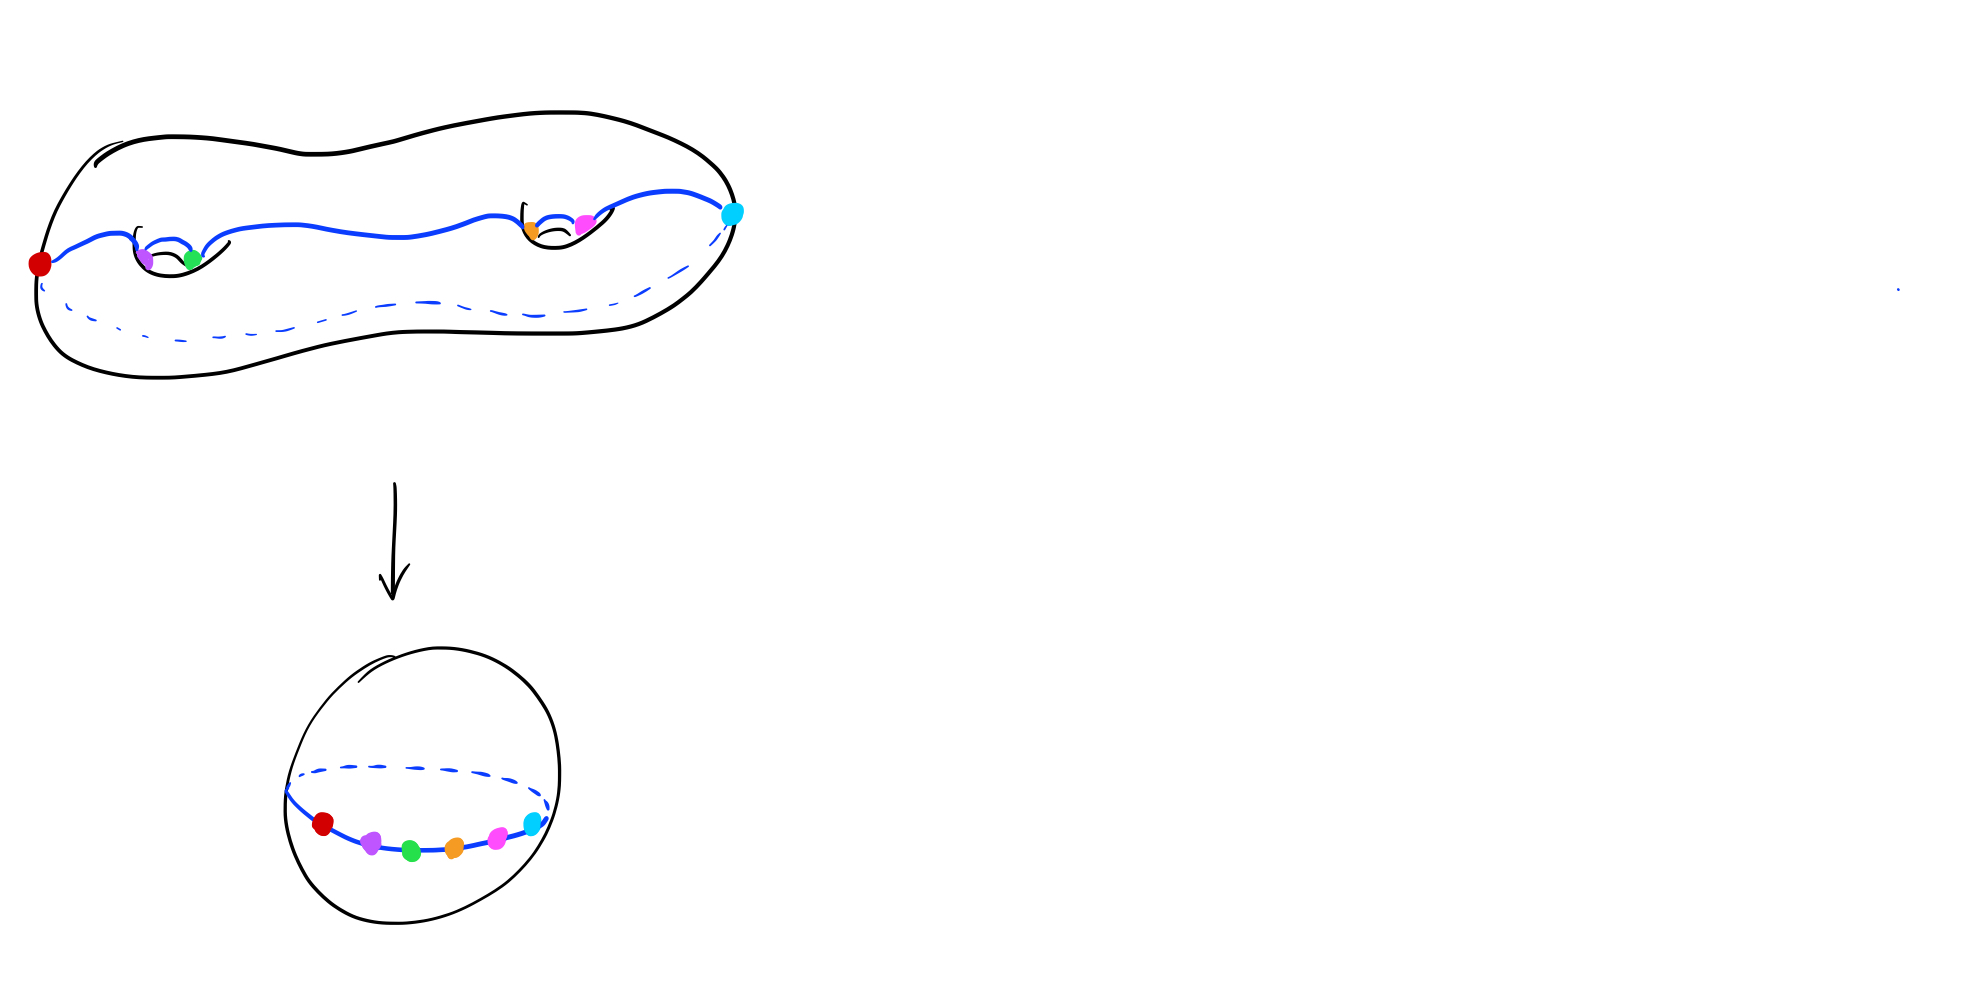
\includegraphics[width=1\linewidth]{fig7}
	\end{figure}
\end{frame}

\begin{frame}{$\LMod(S_{0,6})\cong\Mod(S_{0,6})$}
	\begin{figure}[H]
		\centering
		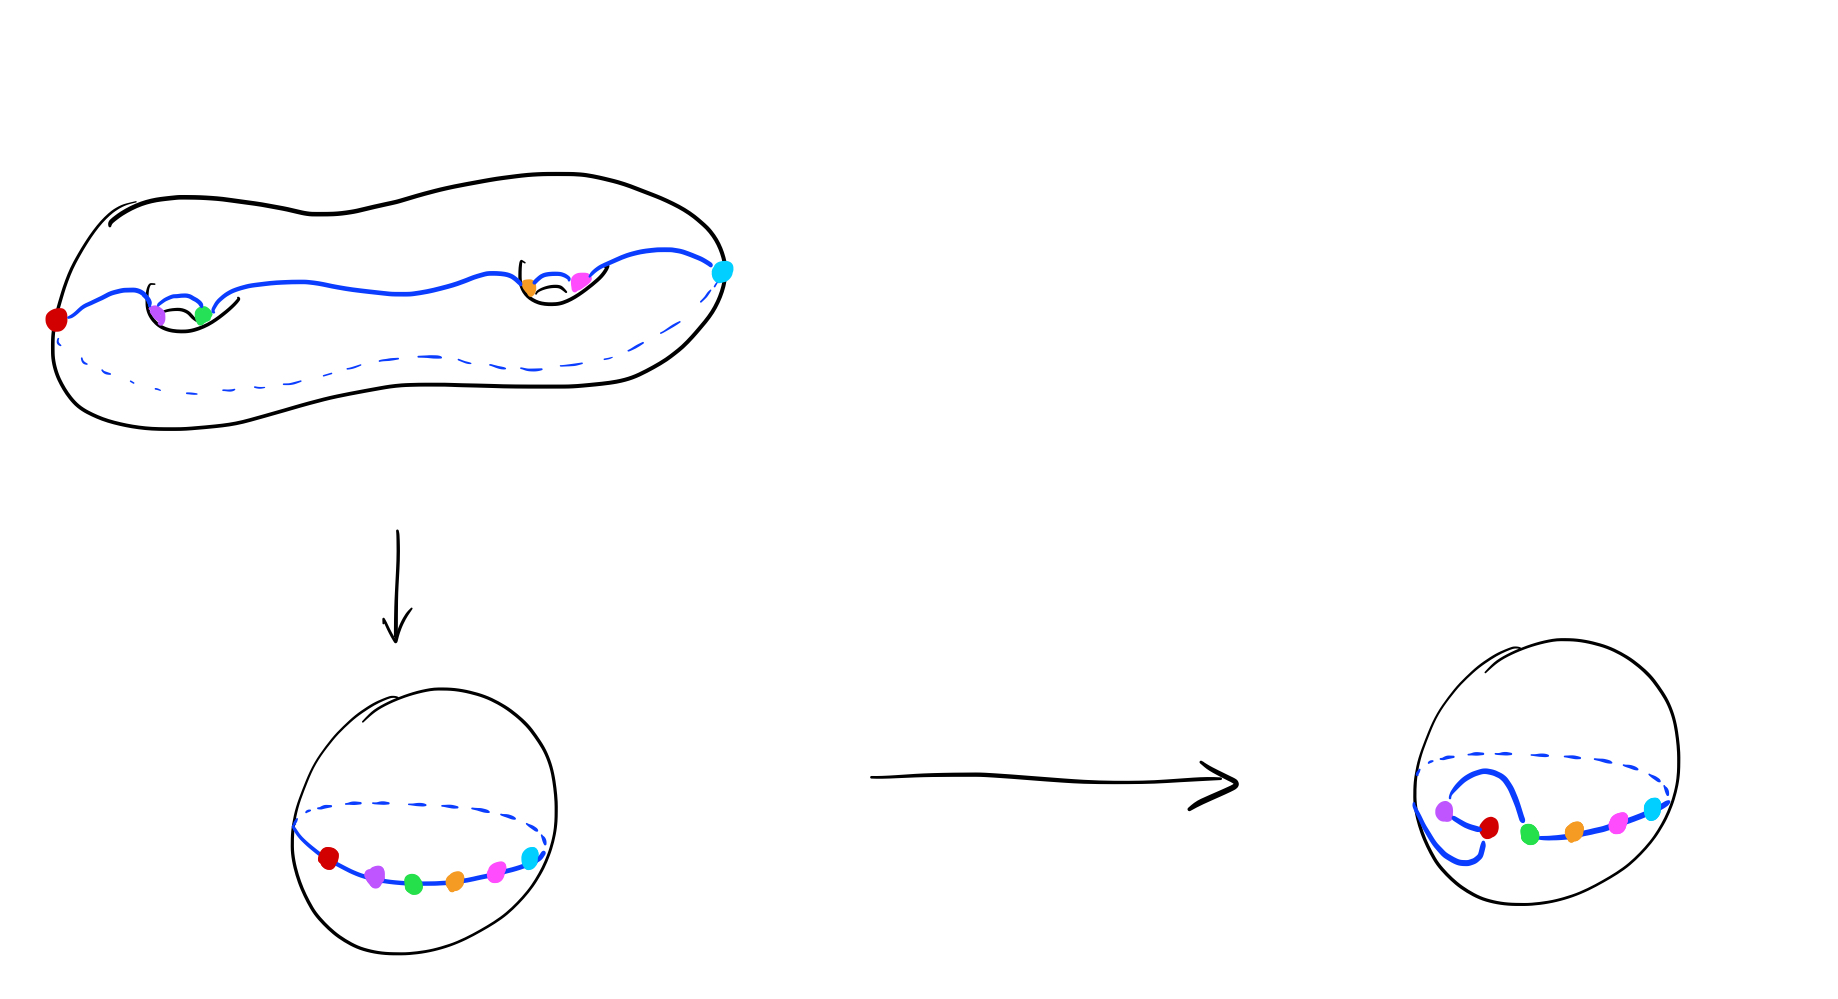
\includegraphics[width=1\linewidth]{fig8}
	\end{figure}
\end{frame}

\begin{frame}{$\LMod(S_{0,6})\cong\Mod(S_{0,6})$}
	\begin{figure}[H]
		\centering
		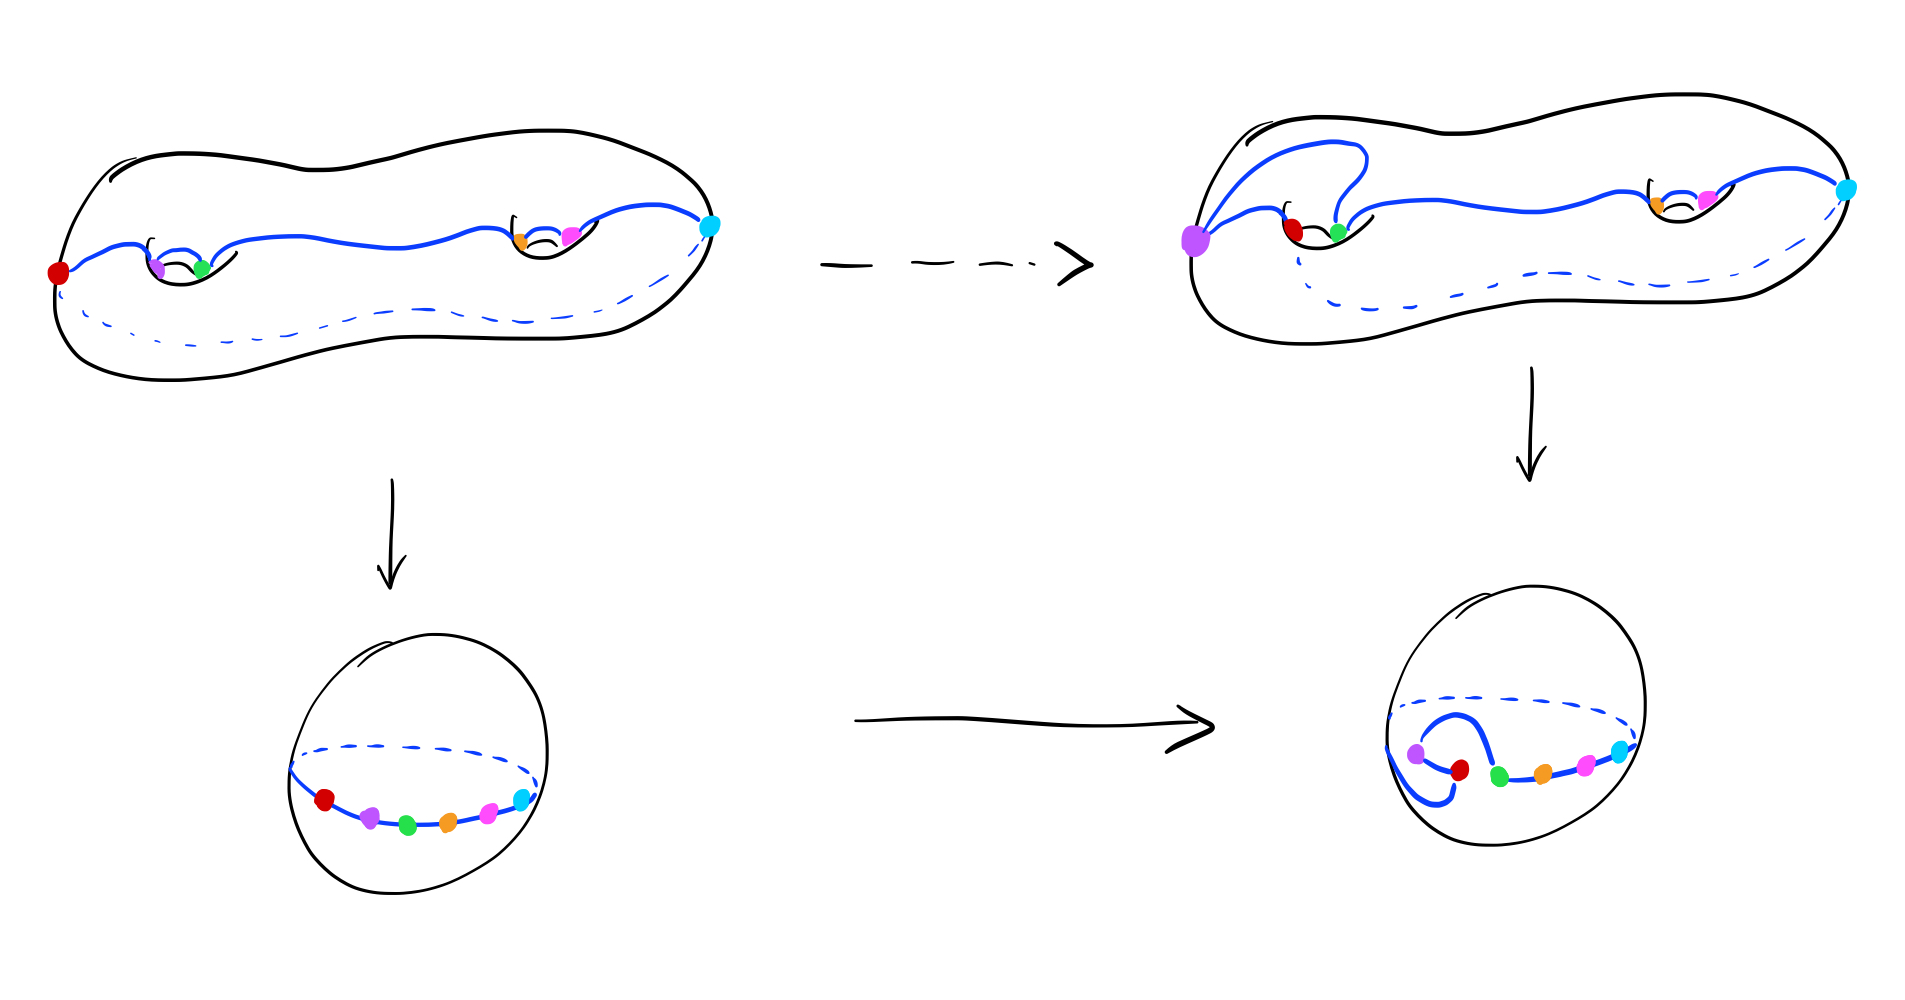
\includegraphics[width=1\linewidth]{fig9}
	\end{figure}
	\pause 
	La observación clave es que los levantamientos de estos medios-giros (la flecha punteada) de hecho son giros de Dehn.
\end{frame}

\begin{frame}{$\LMod(S_{0,6})\cong\Mod(S_{0,6})$}
	\begin{figure}[H]
		\centering
		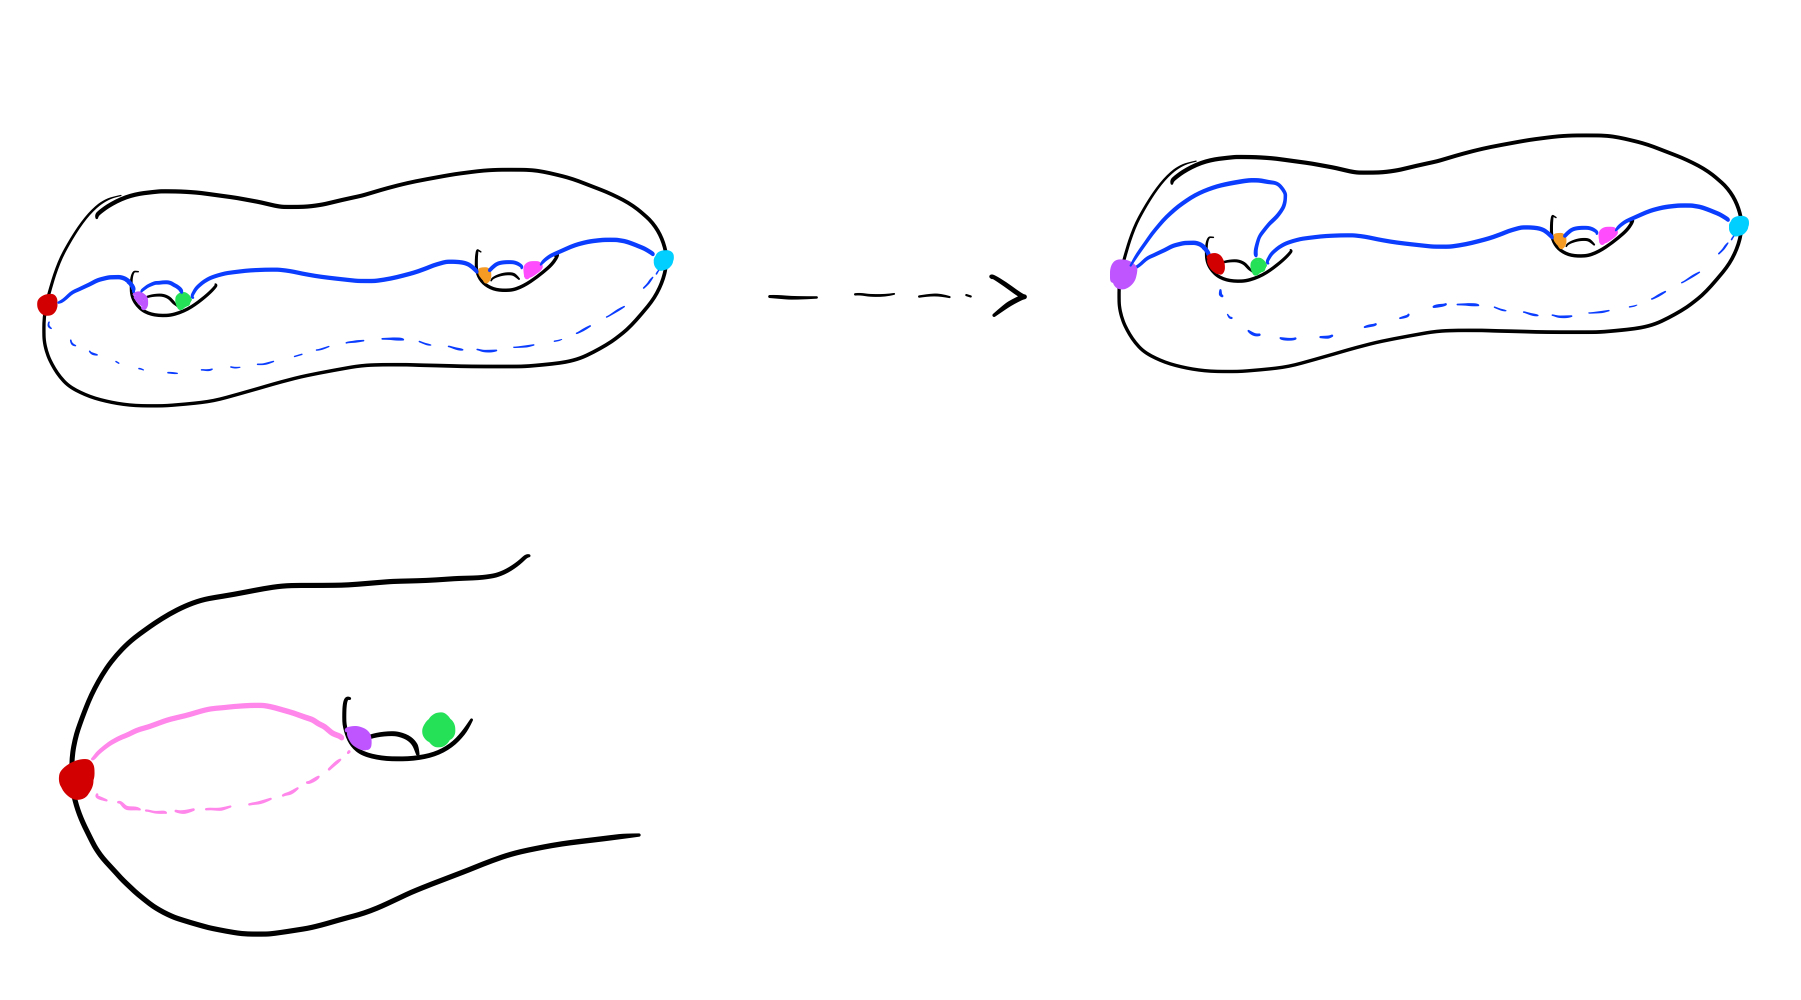
\includegraphics[width=1\linewidth]{fig10}
	\end{figure}
\end{frame}

\begin{frame}{$\LMod(S_{0,6})\cong\Mod(S_{0,6})$}
	\begin{figure}[H]
		\centering
		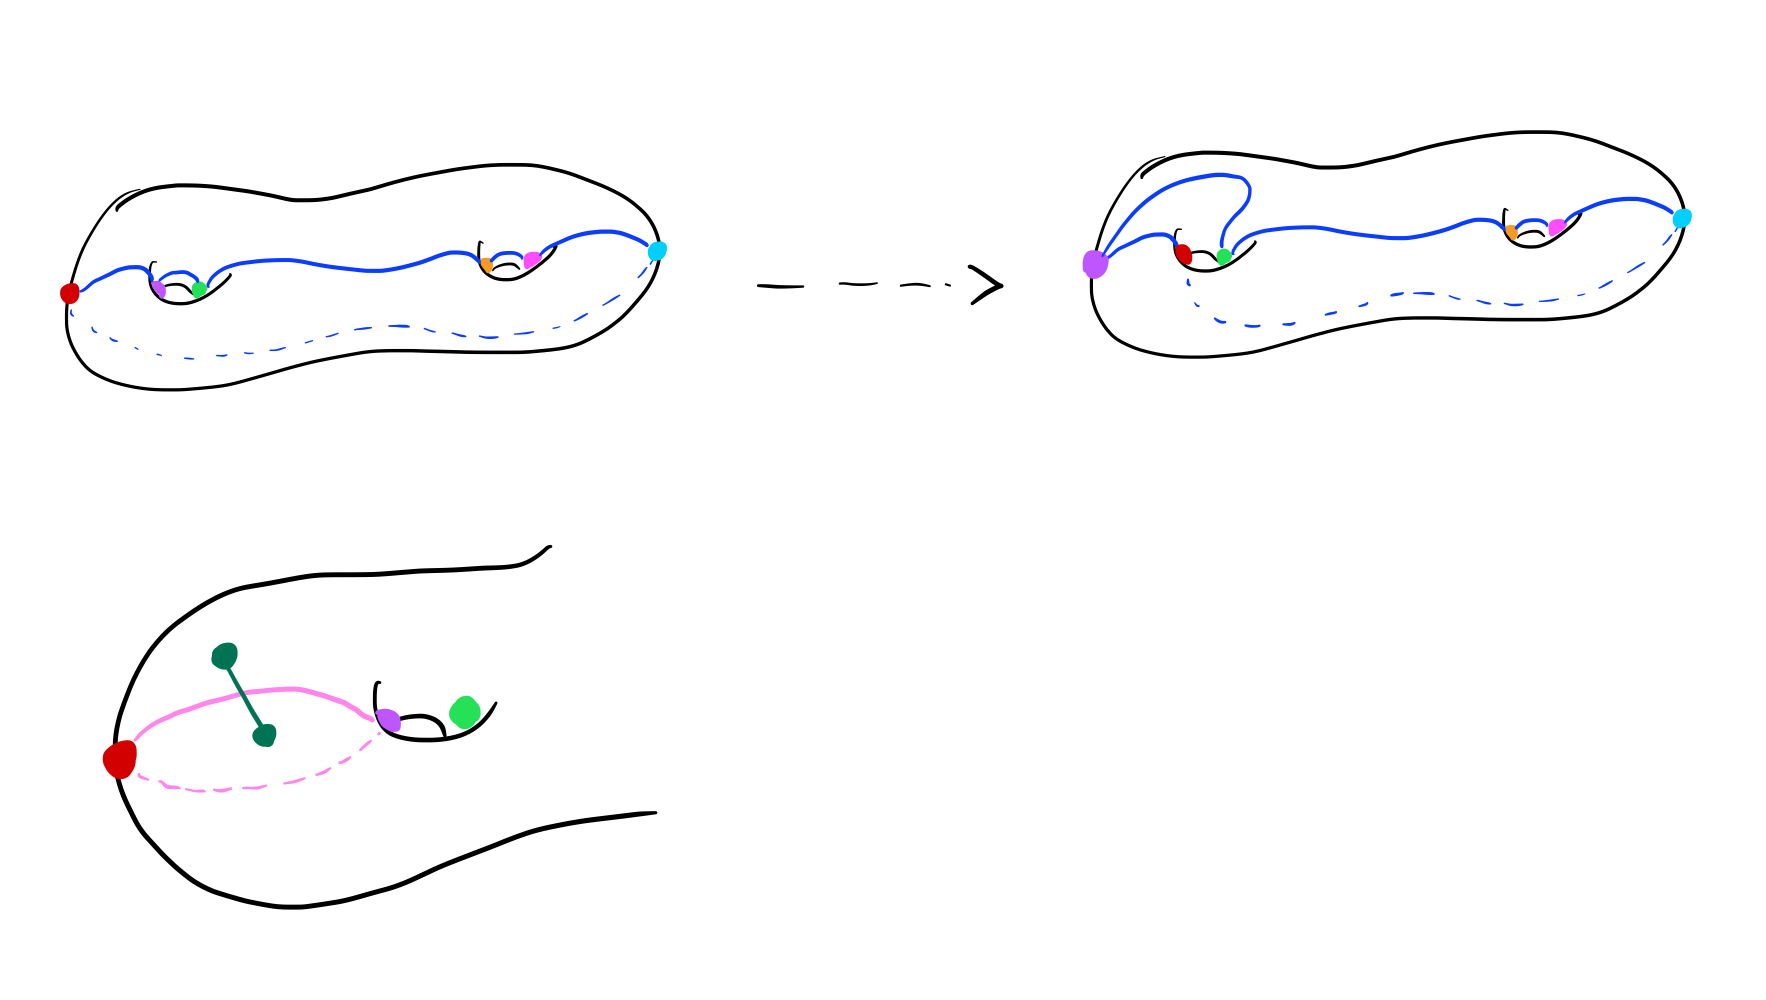
\includegraphics[width=1\linewidth]{fig11}
	\end{figure}
\end{frame}

\begin{frame}{$\LMod(S_{0,6})\cong\Mod(S_{0,6})$}
	\begin{figure}[H]
		\centering
		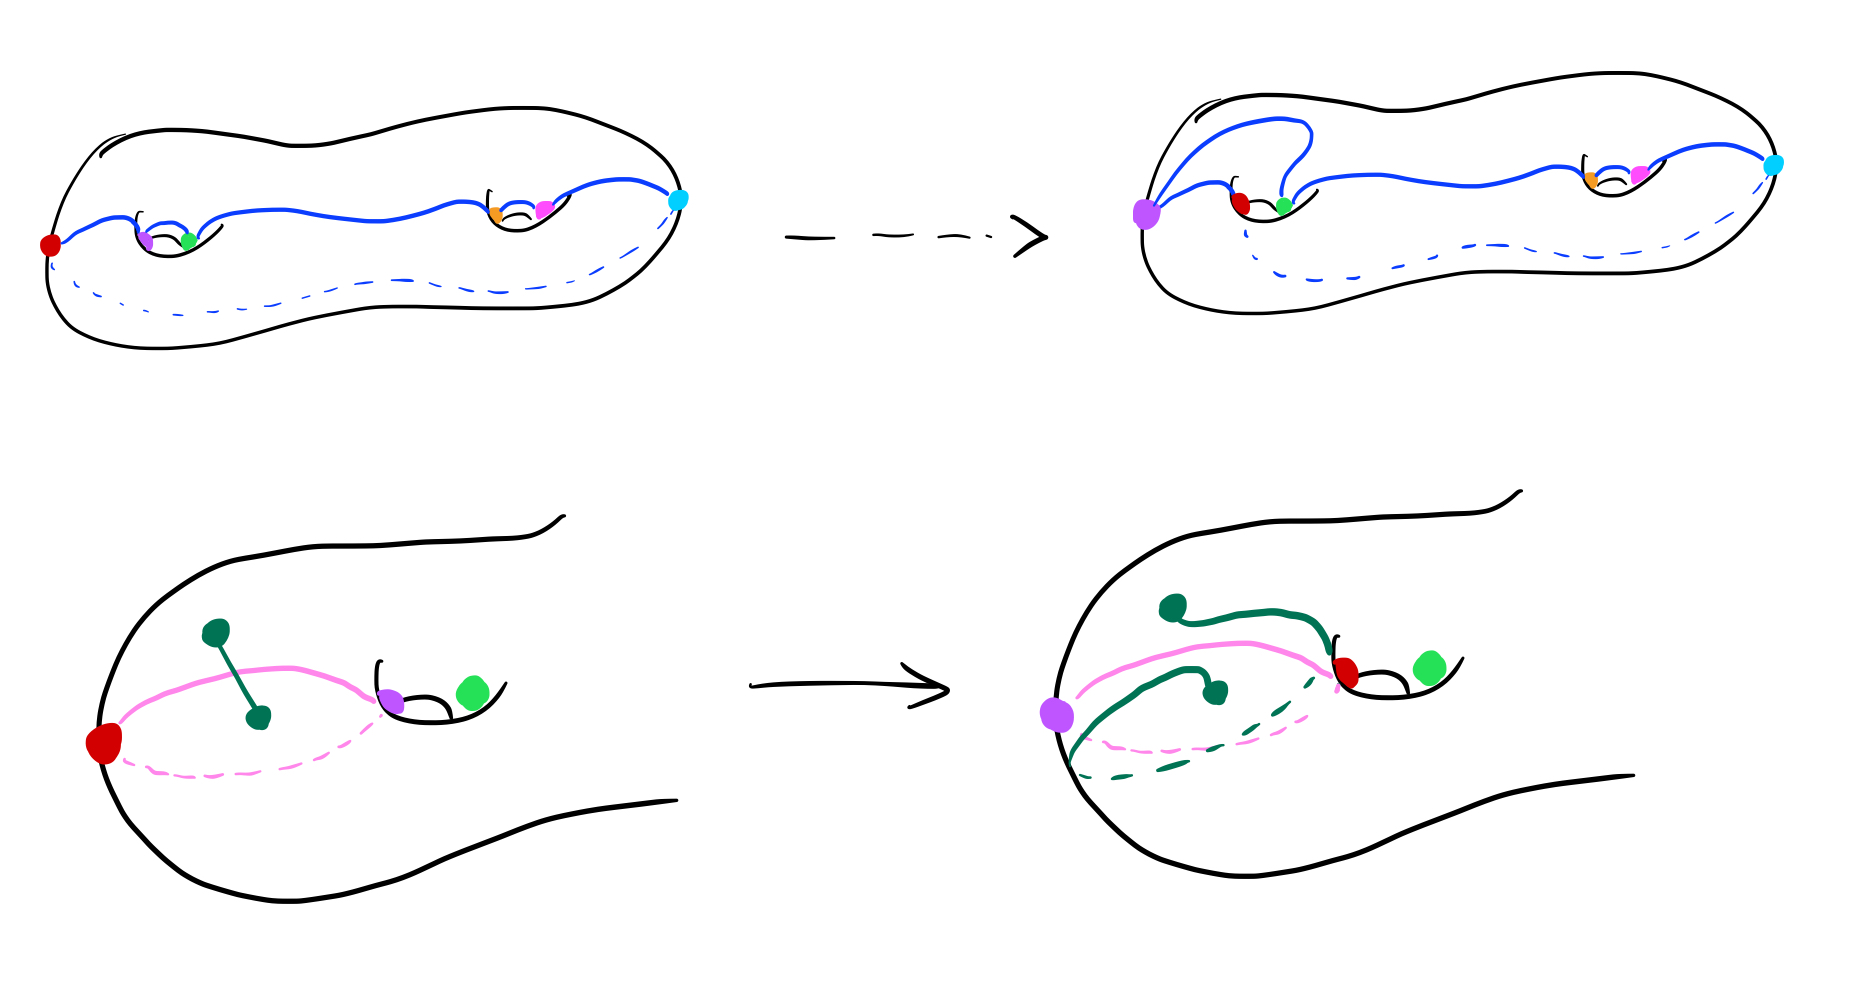
\includegraphics[width=1\linewidth]{fig12}
	\end{figure}
\end{frame}

\begin{frame}{$\LMod(S_{0,6})\cong\Mod(S_{0,6})$}
	\begin{figure}[H]
		\centering
		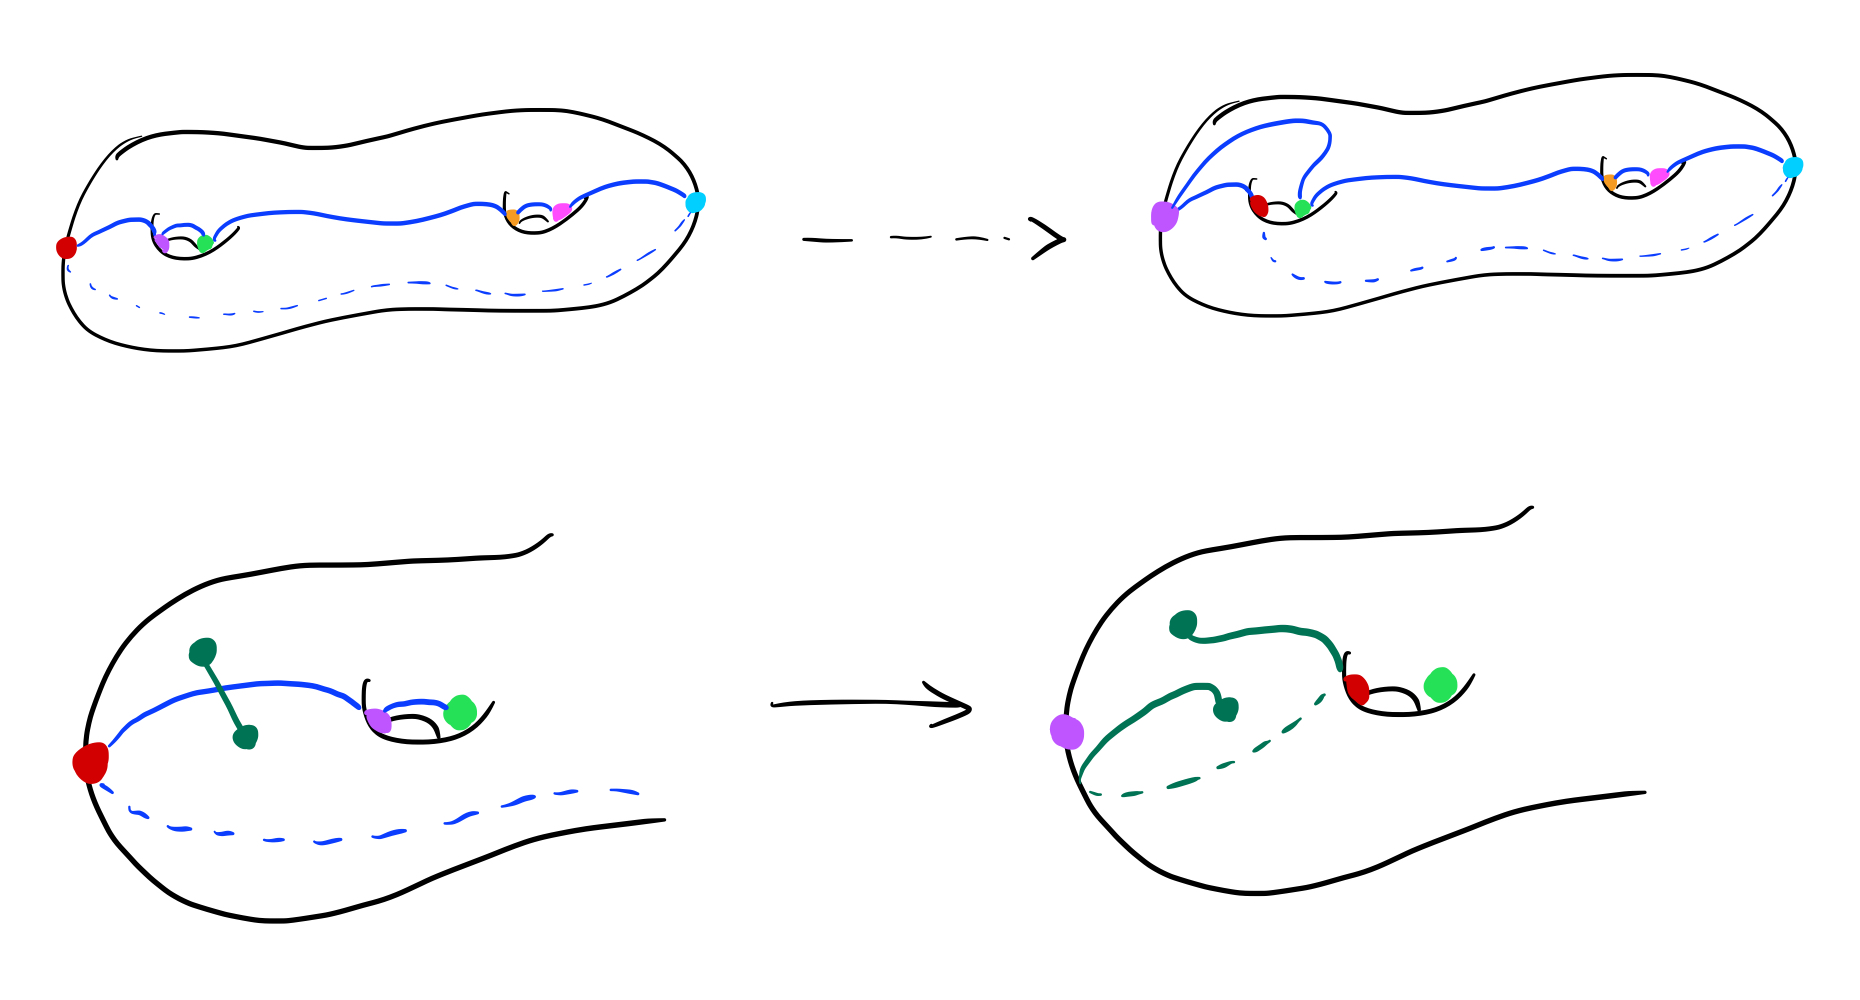
\includegraphics[width=1\linewidth]{fig13}
	\end{figure}
\end{frame}

\begin{frame}{$\LMod(S_{0,6})\cong\Mod(S_{0,6})$}
	\begin{figure}[H]
		\centering
		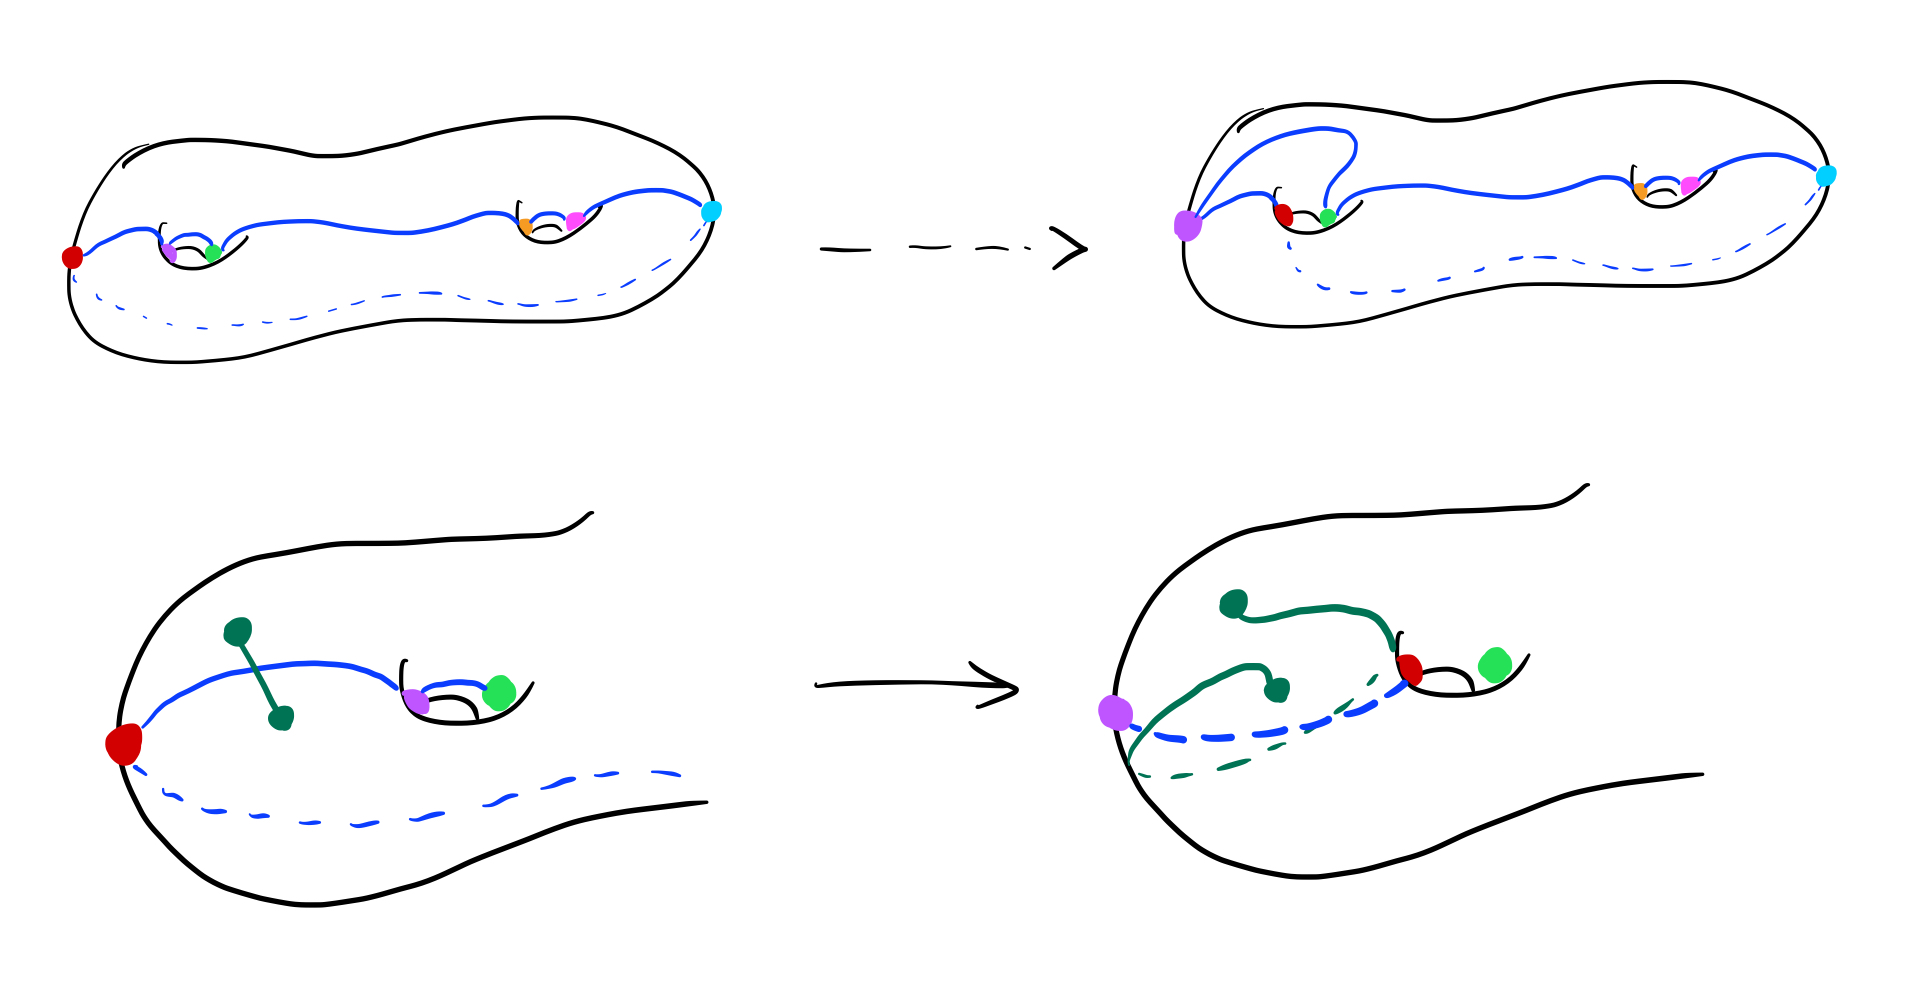
\includegraphics[width=1\linewidth]{fig14}
	\end{figure}
\end{frame}

\begin{frame}{$\LMod(S_{0,6})\cong\Mod(S_{0,6})$}
	\begin{figure}[H]
		\centering
		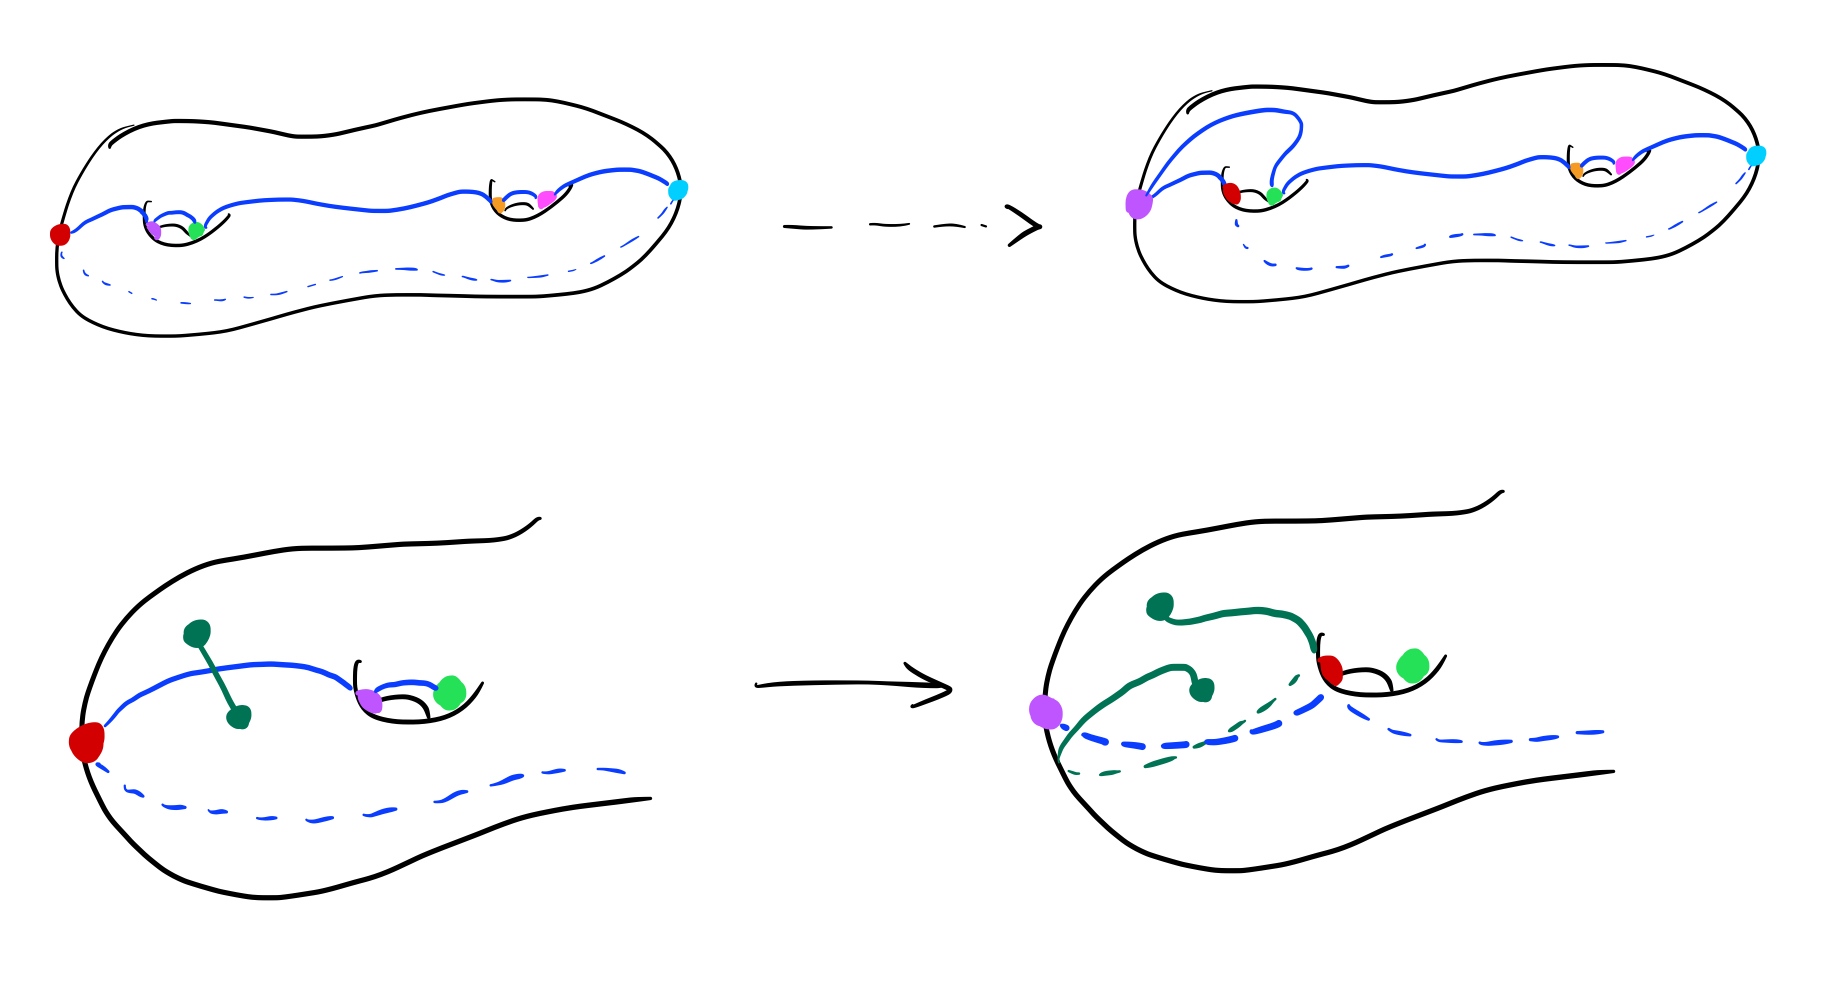
\includegraphics[width=1\linewidth]{fig15}
	\end{figure}
\end{frame}

\begin{frame}{$\LMod(S_{0,6})\cong\Mod(S_{0,6})$}
	\begin{figure}[H]
		\centering
		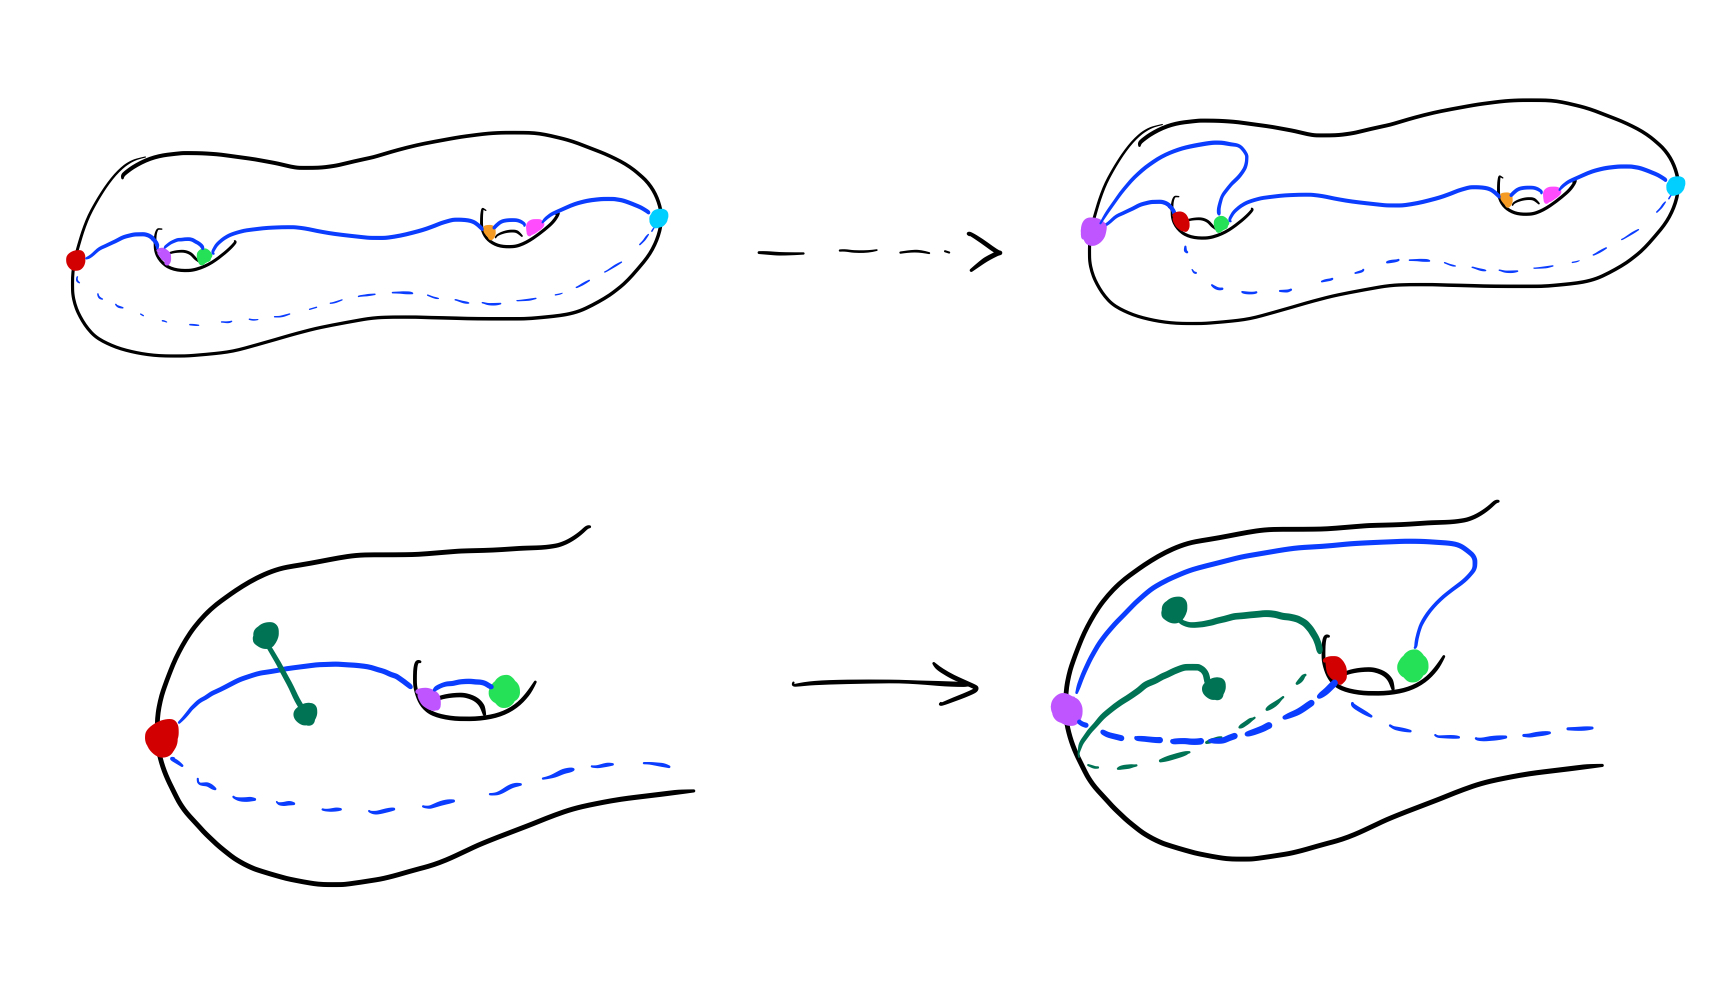
\includegraphics[width=1\linewidth]{fig16}
	\end{figure}\pause
		\begin{center}
		¡El giro de Dehn es un levantamiento del medio giro!
		\end{center}
\end{frame}

\begin{frame}{$\LMod(S_{0,6})\cong\Mod(S_{0,6})$}
	Finalmente concluimos que $\LMod(S_{0,6})\cong\Mod(S_{0,6})$.\pause

	Más aún
	\[\Mod(S_2)/\langle\iota\rangle\approx\Mod(S_{0,6})\]\pause
	Y de hecho, se conoce una presentación de $\Mod(S_{0,6})$.
\end{frame}

\begin{frame}{Una presentación de $\Mod(S_2)$}
	De acuerdo a la presentación de $\Mod(S_{0,6})$ por Magnus, Birman y Hilden encontraron la siguiente presentación para $\Mod(S_2)$ en términos de los generadores de Humphries $T_1$ a $T_5$:
	\begin{align*}
		[T_i,T_j]=1&\qquad \text{para }|i-j|\geq2\\
		T_iT_{i+1}T_i=T_{i+1}T_iT_{i+1}&\qquad\text{para }1\leq i \leq 4\\
		(T_1T_2T_3T_4T_5)^6=1&\\
		(T_1T_2T_3T_4T_5T_5T_4T_3T_2T_1)^2=1&\\
		[T_1T_2T_3T_4T_5T_5T_4T_3T_2T_1,T_1]=1&
	\end{align*}
	\pause Las primeras dos son las relaciones del grupo de trenzas $B_6$, la siguiente describe el kernel de $B_6\to\Mod(S_{0,6})$, y las últimas dos corresponden a la involución hiperelíptica, que es $T_1T_2T_3T_4T_5T_5T_4T_3T_2T_1$.
\end{frame}

\begin{frame}{Una presentación de $\Mod(S_2)$}
	Para ver por qué tenemos esta presentación, notemos que la sucesión exacta
	\[\begin{tikzcd}[ampersand replacement=\&]
		1\arrow[r]\&\langle\iota\rangle\arrow[r,hook]\&\Mod(S_2)\arrow[r,two heads]\&\Mod(S_{0,6})\arrow[r]\&1
	\end{tikzcd}\]
	se escinde por ser $\Mod(S_{0,6})$ un grupo libre, de forma que \[\Mod(S_2)=\langle\iota\rangle\oplus\Mod(S_{0,6})\]
	En general, una presentación del producto directo $G\oplus H$ de dos grupos $G=\langle S_G| R_G\rangle$ y $H=\langle S_H|R_H\rangle$ es $\langle S_G\cup S_H|R_G,R_H, R_P\rangle$ donde $R_P$ son las relaciones de conmutatividad entre cualquier generador de $G$ con cualquier generador de $H$.
\end{frame}

\begin{frame}
	Para verlo rápidamente, notemos que en virtud de las relaciones $R_P$ podemos expresar un elemento en $\langle S_G\cup S_H|R_G,R_H, R_P\rangle$ como el producto de un elemento en $G$ seguido de un elemento en $H$. Esto induce un mapeo natural
	\[\langle S_G\cup S_H|R_G,R_H, R_P\rangle\to \langle S_G| R_G\rangle\oplus \langle S_H|R_H\rangle=G\oplus H\]
	que es suprayectivo y tiene kernel trivial. Para confirmar esto último, tomamos un elemento en el kernel y lo proyectamos a $G$ y a $H$. Como el 
	
	
	%Claramente es suprayectivo. Para ver que su kernel es trivial, tomamos un elemento que vaya a dar a la identidad en $G\oplus H$. Al proyectar en $G$ obtenemos nuevamente el elemento neutro, que debe estar en (la cerradura normal de) $R_G$. Análogamente, la proyección en $H$ es un elemento en $R_H$. Concluimos que el elemento con el que comenzamos es un producto de elementos en $R_G$ y $R_H$, así que a lo más está en $R_P$.
\end{frame}

\begin{frame}
	En \cite{Magnus} ``Combinatorial Group Theory", tenemos:
	
	 \begin{teo}[N9]
	 	$\Mod(S_{0,n})\approx B_n/T_n$ donde $T_n$ está generado por los $n$ elementos $\tau_\nu$ con $\nu=1,\ldots,n-1$ y $\tau$ donde
	 	\begin{align*}
	 		\tau_1&=(\sigma_2\sigma_3\ldots\sigma_{n-1})^{1-n}\\
	 		\tau_2&=\sigma_1^2(\sigma_3\ldots\sigma_{n-1})^{2-n}\\
	 		&\cdots\\
	 		\tau_{\ell+1}&=(\sigma_1\ldots\sigma_\ell)^{\ell+1}(\sigma_{\ell+2}\ldots\sigma_{n+1})^{\ell+1-n}\\
	 		&\cdots\\
	 		\tau_{n-1}&=(\sigma_1\sigma_2\ldots\sigma_{n-2})^{n-1}\\
	 		\tau&=(\sigma_1\sigma_2\ldots\sigma_{n-1})^n
 		\end{align*}
	 \end{teo}
\end{frame}

\begin{frame}
	Así que para $n=6$:

		$\Mod(S_{0,6})\approx B_6/T_6$ donde $T_6$ está generado por
		\begin{align*}
			\tau_1&=(\sigma_2\sigma_3\sigma_4\sigma_{5})^{-5}\\
			\tau_2&=\sigma_1^2(\sigma_3\sigma_4\sigma_{5})^{-4}\\
			\tau_3&=(\sigma_1\sigma_2)^3(\sigma_3\sigma_4\sigma_{5})^{-3}\\
			\tau_4&=(\sigma_1\sigma_2\sigma_3)^4(\sigma_4\sigma_{5})^{-2}\\
			\tau_{5}&=(\sigma_1\sigma_2\sigma_3\sigma_4)^{5}\\
			\tau&=(\sigma_1\sigma_2\sigma_3\sigma_4\sigma_5)^{6}
		\end{align*}
\end{frame}

\begin{frame}
	Ahora nos preguntamos dados un grupo $G=\langle S|R\rangle$ y un subgrupo $T\leq G$ cómo es una presentación de $G/T$. Sólo debemos agregar los elementos de $T$, ya que el mapeo
	\[G\to \langle S|R,T\rangle\]
	tiene kernel $T$. Claro, pues un elemento trivial en el grupo de la derecha es un producto de elementos en la cerradura normal de $R\cup T$, pero los elementos en $R$ se anulan en $G$.
\end{frame}

\begin{frame}
	Como el grupo de trenzas $B_6$ está generado por $\sigma_1,\ldots,\sigma_5$ con las relaciones
	\begin{align*}
		\sigma_i\sigma_j&=\sigma_j\sigma_i\quad \;\;\;\qquad\quad\text{para }|i-j|\geq2\\
		\sigma_i\sigma_{i+1}\sigma_i&=\sigma_{i+1}\sigma_i\sigma_{i+1}\qquad\text{para toda }i
	\end{align*}
	para obtener una presentación de $\Mod(S_{0,6})$ sólo agregamos los generadores $\tau_1$ a $\tau_5$, $\tau$ al conjunto de relaciones.
	
	\pause Más aún, para tener una presentación de $\Mod(S_2)$ sólo debemos agregar la involución hiperelíptica $\iota$ elevada al cuadrado, y los conmutadores de $\iota$ con los generadores de $\Mod(S_{0,6})$.
\end{frame}

\iffalse
\begin{frame}
	Ahora nos preguntamos dados un grupo $G=\langle S_G|R_G\rangle$ y un subgrupo $T=\langle S_T|R_T\rangle\leq G$ cómo es una presentación de $G/T$. Sólo debemos agregar las relaciones de $T$, ya que el mapeo
	\[G\to \langle S_G|R_G,R_T\rangle\]
	tiene kernel $T$, ya que un elemento trivial en el grupo de la derecha es un producto de elementos en la cerradura normal de $R_G\cup R_T$, y los elementos en $R_G$ se anulan en $G$.
\end{frame}

\begin{frame}
	Como el grupo de trenzas $B_6$ está generado por $\sigma_1,\ldots,\sigma_5$ con las relaciones
	\begin{align*}
		\sigma_i\sigma_j&=\sigma_j\sigma_i\quad \;\;\;\qquad\quad\text{para }|i-j|\geq2\\
		\sigma_i\sigma_{i+1}\sigma_i&=\sigma_{i+1}\sigma_i\sigma_{i+1}\qquad\text{para toda }i
	\end{align*}
	para obtener una presentación de $\Mod(S_{0,6})$ sólo agregamos los generadores $\tau_1$ a $\tau_5$, $\tau$.
	
	\pause Más aún, para tener una presentación de $\Mod(S_2)$ sólo debemos agregar la involución hiperelíptica $\iota$ con su relación, y los conmutadores de $\iota$ con los generadores de $\Mod(S_{0,6})$.
\end{frame}\fi

\begin{frame}{Una presentación de $\Mod(S_2)$}
	Veamos de nuevo la presentación que está en el artículo:
	  
	si $T_1$ a $T_5$ son los generadores de Humphries,
	\begin{align*}
		[T_i,T_j]=1&\qquad \text{para }|i-j|\geq2\\
		T_iT_{i+1}T_i=T_{i+1}T_iT_{i+1}&\qquad\text{para }1\leq i \leq 4\\
		(T_1T_2T_3T_4T_5)^6=1&\\
		(T_1T_2T_3T_4T_5T_5T_4T_3T_2T_1)^2=1&\\
		[T_1T_2T_3T_4T_5T_5T_4T_3T_2T_1,T_1]=1&
	\end{align*}
\end{frame}

\begin{frame}{Una presentación de $\Mod(S_2)$}
	Con la notación de grupo de trenzas:
	\begin{align*}
		[\sigma_i,\sigma_j]=1&\qquad \text{para }|i-j|\geq2\\
		\sigma_i\sigma_{i+1}\sigma_i=\sigma_{i+1}\sigma_i\sigma_{i+1}&\qquad\text{para }1\leq i \leq 4\\
		\tau=1&\\
		\iota^2=1&\\
		[\iota,\sigma_1]=1&
	\end{align*}
	¿Dónde están $\tau_1$ a $\tau_5$ y los demás conmutadores?
\end{frame}

\begin{frame}{Una presentación de $\Mod(S_2)$}
	Veamos si podemos comprobar que $[\iota,\sigma_2]$.\pause 
	\begin{align*}
		T_1T_2T_3T_4T_5T_5T_4T_3T_2T_1\cdot T_2&=T_1T_2T_3T_4T_5T_5T_4T_3T_2T_1 T_2\\
		&=T_1T_2T_3T_4T_5T_5T_4T_3\textcolor{magenta}{T_1T_2 T_1}\\
		&=T_1T_2\textcolor{blue}{T_1}T_3T_4T_5T_5T_4T_3T_2T_1\\
		&=\textcolor{orange}{T_2T_1T_2}T_3T_4T_5T_5T_4T_3T_2T_1\\
		&=T_2\cdot T_1T_2T_3T_4T_5T_5T_4T_3T_2T_1
	\end{align*}
	\pause Este truco funciona para $[\iota,\sigma_3]$, $[\iota,\sigma_4]$ y $[\iota,\sigma_5]$.
	
	\pause 	En el artículo de Margalit y Winarski se afirma que la relación $\tau$	\textit{describe el kernel del mapeo $B_6\to \Mod(S_{0,6})$}, lo que explicaría por qué no están incluidas las relaciones $\tau_1$ a $\tau_5$.
\end{frame}

\section{Generalización para $\SMod(S_g)$}

\begin{frame}{Grupo de trenzas}
	\pause Dados $p_1,\ldots,p_n\in\C$, el \textbf{\textit{grupo de trenzas}} $B_n$ consiste de las clases de isotopía de $n$ caminos $f_i:[0,1]\to\C\times[0,1]$ tales que $f_i[0,1]$ son disjuntos, $f_i(0)=p_i$, $f_i(1)=p_{\bar{f}(i)}$ y $f_i(t)\in\C\times\{t\}$ para alguna permutación de $n$ elementos $\bar{f}$. Este grupo está generado por $n-1$ elementos que satisfacen las siguientes relaciones:
	\begin{align*}
		\sigma_i\sigma_j&=\sigma_j\sigma_i\quad \;\;\;\qquad\quad\text{para }|i-j|\geq2\\
		\sigma_i\sigma_{i+1}\sigma_i&=\sigma_{i+1}\sigma_i\sigma_{i+1}\qquad\text{para toda }i
	\end{align*}
\end{frame}



\begin{frame}{Grupo de trenzas}
%	Si $D_n$ es el disco $D^2$ con $n$ puntos marcados, tenemos el siguiente isomorfismo:
%	\[B_n\approx \Mod(D_n)\]
	Para encontrar una propiedad interesante del grupo de trenzas, consideremos el disco $D^2$ con $n$ puntos marcados, $D_n$.
	
	\pause Un elemento de $\Mod(D_n)$ puede ser pensado como un homeomorfismo del disco en sí mismo. \pause Sabemos que $\Mod(D^2)\approx1$, de forma que hay una isotopía con la identidad. \pause En cada momento de la isotopía, los de puntos marcados se mueven en el interior del disco y vuelven al punto inicial, de manera que tenemos una trenza.
\end{frame}

\begin{frame}{Grupo de trenzas}

	\begin{figure}[H]
		\centering
		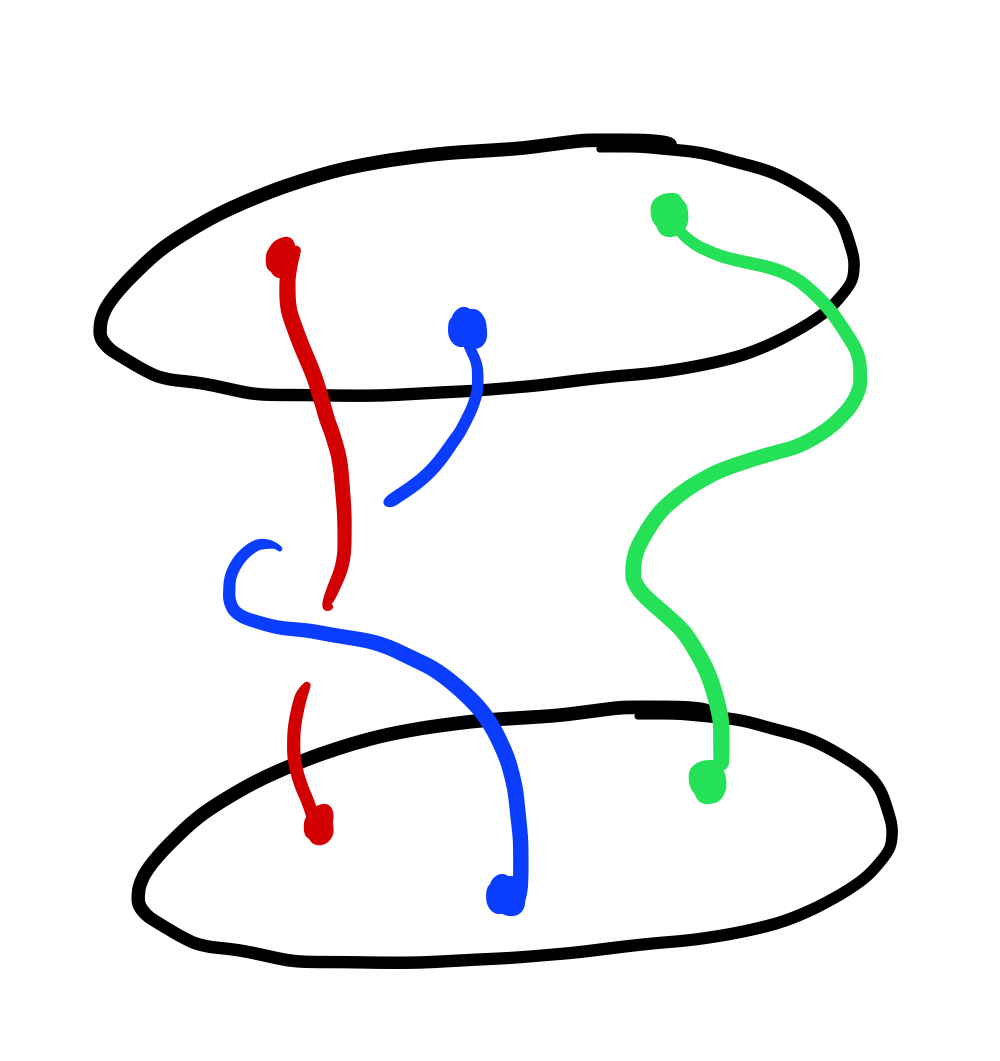
\includegraphics[width=0.4\linewidth]{fig27}
	\end{figure}
	\pause De hecho,
	\[B_n\approx \Mod(D_n)\]
	La demostración de que esta correspondencia es un isomorfismo se obtiene de una generalización de la sucesión exacta de Birman.
\end{frame}

\begin{frame}{Una presentación para $\SMod(S_g)$}
	\pause Birman y Hilden mostraron la siguiente presentación para $\SMod(S_g)$. Dados los generadores $t_1,\ldots,t_{n-1}$, las relaciones son
	\begin{align*}
		[t_i,t_j]=1,&\qquad i,j=1,\ldots,n-1\text{ t.q. }|i-j|\geq2\\
		t_it_{i+1}t_i=t_{i+1}t_it_{i+1},&\qquad i=1,\ldots,n-2\\
		(t_1t_2\ldots t_{n-1})^n=1&\\
		(t_1t_2\ldots t_{n-1}t_{n-1}\ldots t_2t_1)^k=1&\\
		[t_1t_2\ldots t_{n-1}t_{n-1}\ldots t_2t_1,t_1]=1&
	\end{align*}
	\pause
	donde, en casos más generales, $2g=(k-1)(n-2)$. Si $n=2g+2$ es la cantidad de puntos marcados, tenemos simplemente que $k=2$.
\end{frame}

\begin{frame}{Una presentación para $\Mod(S^1_g)$}
	Veamos rápidamente qué pasa con la superficie de género $g$ con una componente frontera, $S^1_g$.
	%\[\SMod(S^1_g)\approx B_{2g+1}\]\pause
	\pause En este caso el cociente bajo $\iota$ es un disco con $2g+1$ puntos marcados:
	\begin{figure}[H]
		\centering
		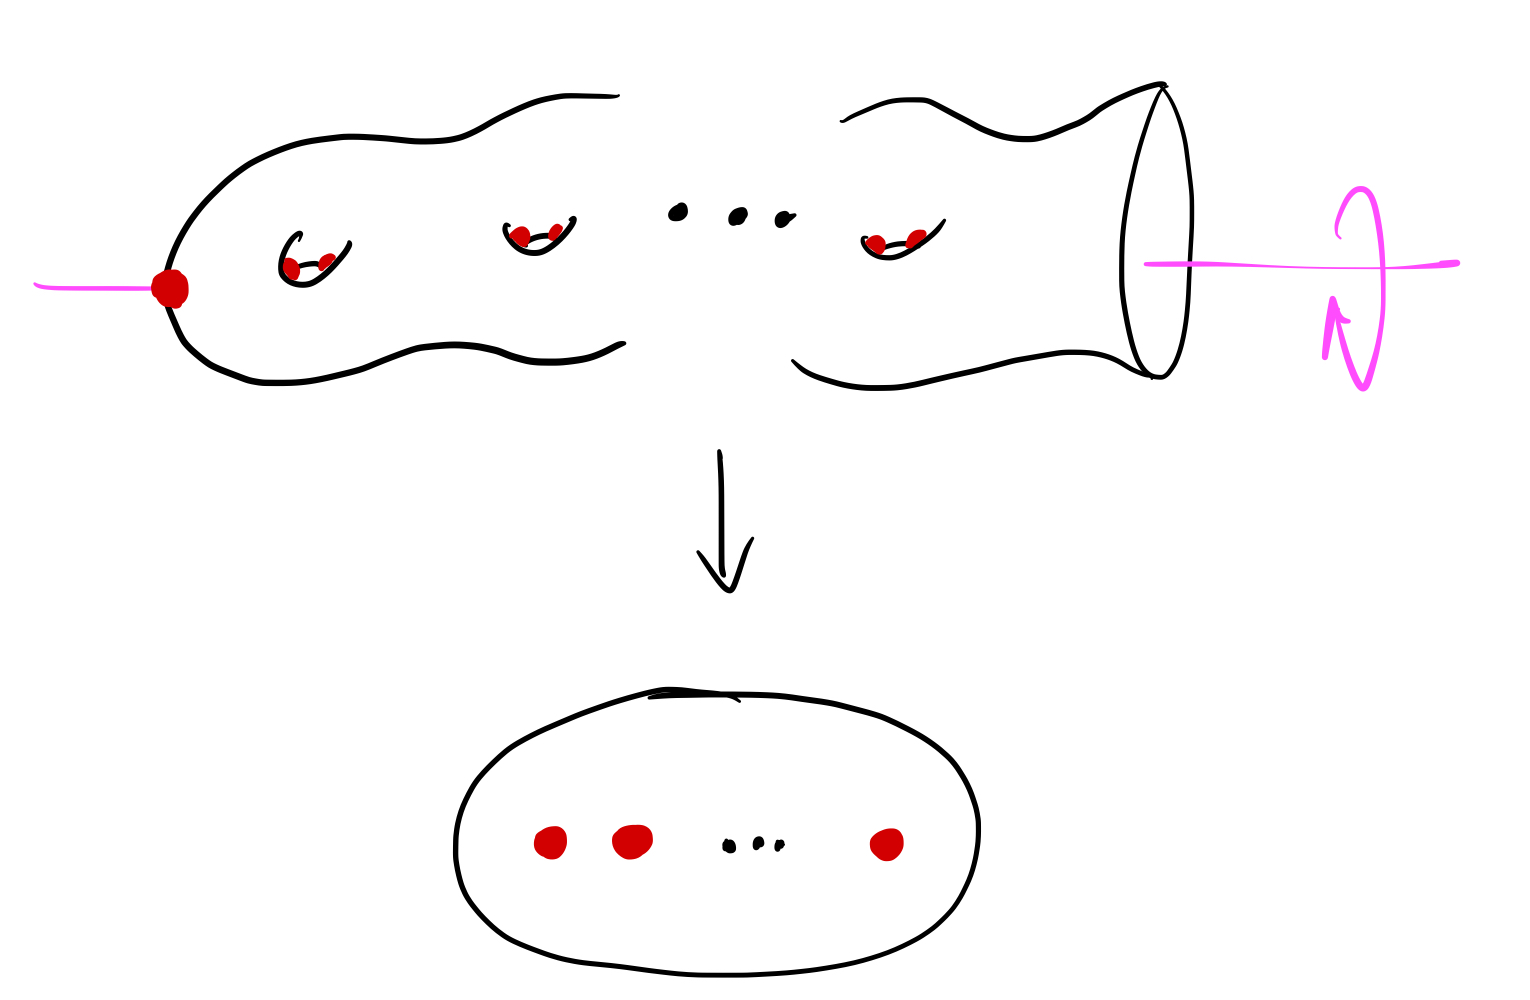
\includegraphics[width=0.6\linewidth]{fig25}
	\end{figure}
\end{frame}

\begin{frame}{Una presentación para $\Mod(S^1_g)$}
\begin{figure}[H]
	\centering
	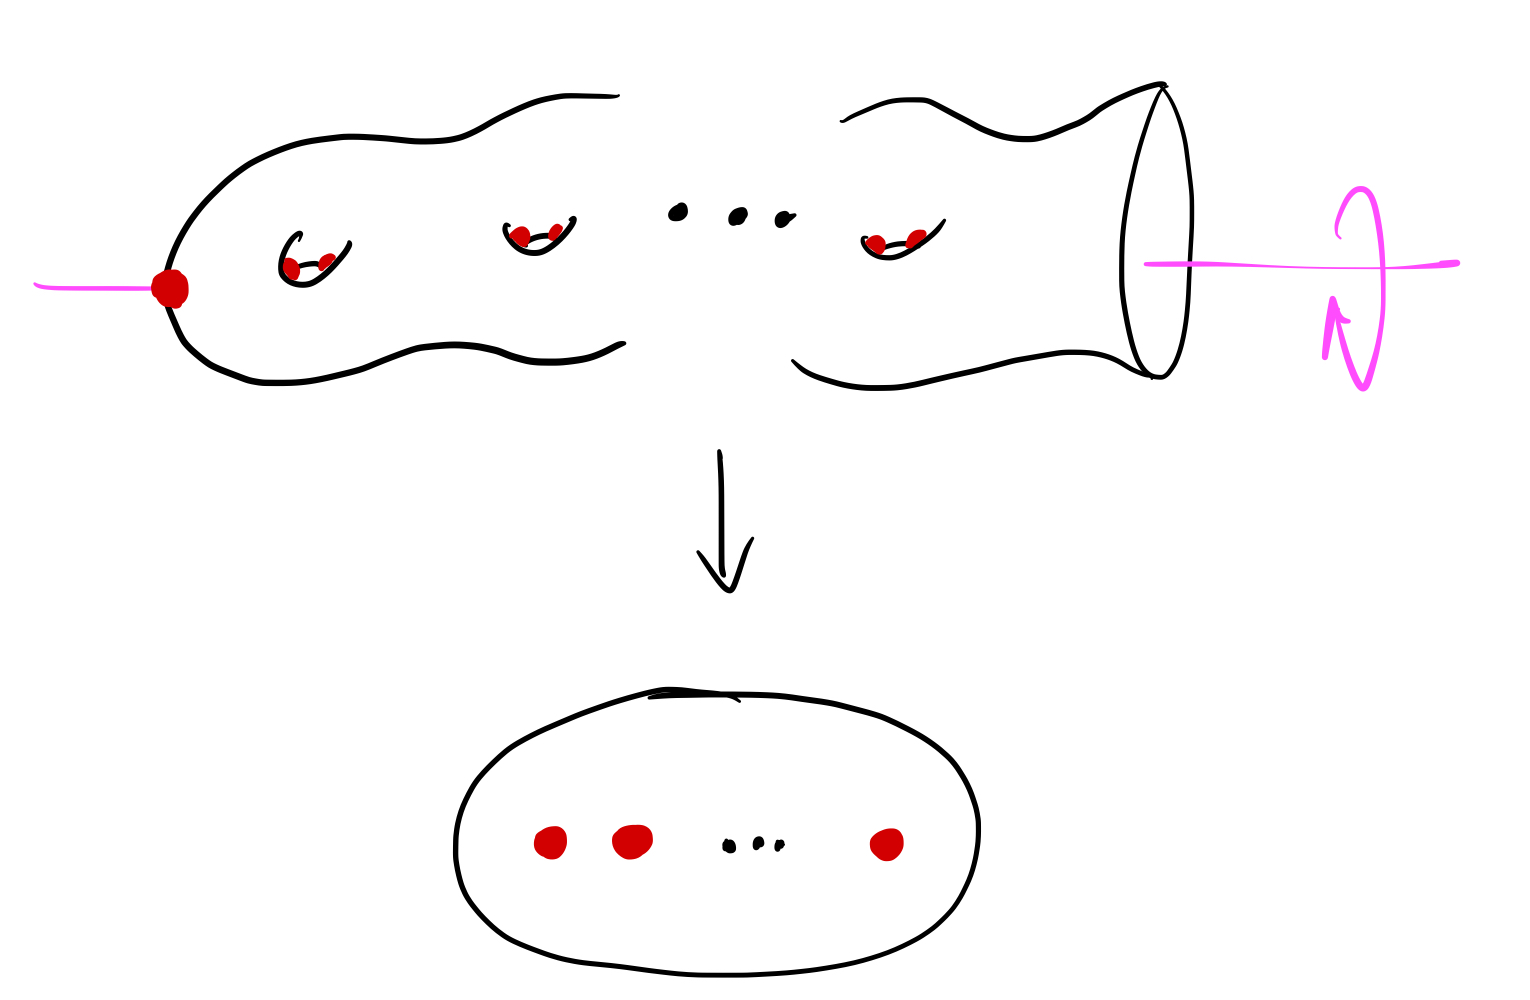
\includegraphics[width=0.6\linewidth]{fig25}
\end{figure}
	Por el teorema de Birman-Hilden, las homotopías en $S_g^1$ pasan al cociente, y además los homeomorfismos del disco punteado son levantables, \pause así que
	\[\SMod(S^1_g)\approx\Mod(D_{2g+1})\pause \approx B_{2g+1}\]
\end{frame}

	\section{Aplicaciones\\
	{\small La signatura de una 4-variedad}}
\begin{frame}{La signatura de una 4-variedad}
	La \textbf{\textit{signatura de una 4-variedad}} $M$ conexa y orientada es la signatura de la forma cuadrática inducida por el producto copa en $H^2(M;\R)$. \pause Recordemos que el producto copa es un operador
	\begin{align*}
		\smile:H^p(M;\R)\times H^{q}(M;\R)\to H^{p+q}(M;\R)
	\end{align*}
	en los grupos de cohomología, obtenidos de dualizar el complejo de cadenas singulares.
\end{frame}

\begin{frame}{La signatura de una 4-variedad}
	En particular, podemos pensarlo en
	\begin{align*}
		\smile:H^k(M;\R)\times H^{n-k}(M;\R)\to H^{n}(M;\R)
	\end{align*}
	\pause Como los $n$-cociclos son homomorfismos $H_n(M;\R)\to\R$, podemos calcular
	\[\alpha\smile\beta([M])\]
	donde $[M]$ es la clase fundamental dada por la orientación de $M$.
\end{frame}

\begin{frame}{La signatura de una 4-variedad}
	El mapeo resultante es el \textbf{\textit{apareamiento del producto copa}},
	\begin{align*}
		\smile:H^k(M;\R)\times H^{n-k}(M;\R)&\to \R\\
		(\alpha,\beta)&\mapsto \alpha\smile\beta([M])
	\end{align*}
	\pause que es un operador no degenerado en el sentido de que $\alpha\smile\beta=0$ para toda $\beta\in H^{n-k}(M;\R)$ implica $\alpha=0$, y análogamente para $\beta$. \pause Este tipo de operadores están en biyección con las \textbf{\textit{formas bilineales simétricas}}.
\end{frame}

\begin{frame}{La signatura de una 4-variedad}
	Por la \textbf{\textit{ley de inercia de Sylvester}}, la cantidad de números positivos, negativos y cero en cualquier matriz diagonalizada asociada a una forma bilineal simétrica es invariante bajo cambios de base.\pause
	
	La \textbf{\textit{signatura de una forma cuadrática}} $Q$ es $\sigma(Q)=n_++n_-$ donde cualquier matriz diagonal que represente a $Q$ tiene $n_+$ entradas positivas y $n_-$ entradas negativas.\pause
	
	La \textbf{\textit{signatura de una 4-variedad}} $M$ es la signatura del operador $\smile$ que hemos definido.
\end{frame}

\begin{frame}{La signatura de una 4-variedad}
	Interesantemente,
	\[\operatorname{Sign}(X\times Y)=\operatorname{Sign}(X)\operatorname{Sign}(Y)\]
	definiendo la signatura $\operatorname{Sign}(X)=0$ si la dimensión de $X$ no es divisible entre 4.
	
	\pause ¿Es posible reemplazar $X\times Y$ por un haz fibrado con base $X$ y fibra $Y$?
\end{frame}

\begin{frame}{La signatura de una 4-variedad}
Un \textbf{\textit{haz fibrado}} en un espacio $E$ con base $B$ y fibra $F$ es una proyección $p:E\to B$ tal que para cada $x\in B$ hay una vecindad $U$ y un homeomorfismo $h:p^{-1}(U)\to U\times F$ tal que el siguiente diagrama conmuta:
\[\begin{tikzcd}[ampersand replacement=\&]
	p^{-1}(U)\arrow[r,"h"]\arrow[d,"p",swap]\&U\times F\arrow[ld]\\
	U
\end{tikzcd}\]
donde la flecha de la derecha es la proyección al primer factor. \pause Se trata de una correspondencia que a cada punto de $U$ asocia una copia de $F$. Por ejemplo, el \textbf{\textit{haz tangente}} es un haz fibrado cuya fibra es el espacio tangente.
\end{frame}

\begin{frame}{La signatura de una 4-variedad}
	En la fórmula
	\[\operatorname{Sign}(X\times Y)=\operatorname{Sign}(X)\operatorname{Sign}(Y)\]
\textbf{no siempre} es posible reemplazar $X\times Y$ por un haz fibrado con base $X$ y fibra $Y$. ¿Cuáles serán las condiciones necesarias?

\pause En `The signature of fibre-bundles', \cite{Atiyah} muestra un co`ntraejemplo dado por un \textbf{\textit{haz de superficies}} en una superficie, un haz fibrado cuya base y fibra son superficies, que tiene estructura de 4-variedad. \pause La condición clave es que \textit{la acción del grupo fundamental de $X$ actúe trivialmente en la cohomología de $Y$}.

\pause En este contexto, Meyer mostró que si un haz de superficies sobre una superficie tiene \textbf{\textit{monodromía}} en $\SMod(S_g)$, entonces la signatura de la 4-variedad que resulta es cero.

 %La \textbf{\textit{monodromía}} es un grupo que se asocia a los levantamientos de caminos en un cubriente de superficies de Riemann. Intuitivamente, para un cubriente de grado $d$, el levantamiento de un lazo en el espacio base induce una permutación de $d$ elementos dada por el punto inicial y el punto final. Así, el grupo fundamental del espacio base menos los puntos de ramificación tiene una representación en el grupo simétrico de $d$ elementos.
\end{frame}

\begin{frame}
	\begin{defn}
		\begin{itemize}
			\item Sea $G$ un grupo topológico (un espacio topológico con estructura de grupo tal que la operación de grupo y la inversión son funciones continuas) que actúa \textbf{libre}, \textbf{propia} y \textbf{continuamente} en un espacio contraible $X$. Decimos que $X/G$ es un \textbf{espacio clasificante de $G$}. Denotaremos $X/G=BG$ y $X=EG$.
			
			\pause \item Un espacio $X$ que tiene sólo un grupo de homotopía no trivial $\pi_n(X)\approx G$ es un \textbf{espacio de Eilenberg-MacLane}.
		\end{itemize}
	\end{defn}
	\pause \begin{obs}
		Si $G$ es un grupo discreto (todos los puntos son conjuntos abiertos), entonces $BG$ es un espacio $K(G,1)$.
	\end{obs}
	\end{frame}

\begin{frame}{La signatura de una 4-variedad}
	Consideremos el siguiente haz fibrado:
	\textcolor{magenta}{
	\[\begin{tikzcd}[ampersand replacement=\&]
		\Homeo_0(S_g)\arrow[r]\&\Homeo^+(S_g)\arrow[r,"\pi"]\&\Mod(S_g)
	\end{tikzcd}\]}
	cuyas fibras son copias de la mapping class trivial \[\Homeo_0(S_g)=\{f\in\Homeo(S_g):f\simeq\Id\}\]
	\pause Por la \textbf{sucesión exacta de homotopía}, $\pi$ induce un isomorfismo en todos los grupos de homotopía. 
\end{frame}

\begin{frame}
		\textcolor{magenta}{
		\[\begin{tikzcd}[ampersand replacement=\&]
			\Homeo_0(S_g)\arrow[r]\&\Homeo^+(S_g)\arrow[r,"\pi"]\&\Mod(S_g)
		\end{tikzcd}\]}
	\begin{teo}[Whitehead]
		Sea $f:X\to Y$ una función continua entre dos complejos CW. Si $f_*:\pi_n(X)\to\pi_n(Y)$ es un isomorfismo para toda $n$, entonces $f$ es una equivalencia homotópica.
	\end{teo}
	\pause
	Por este teorema, concluimos que $\pi$ es una equivalencia homotópica, donde $\Mod(S)$ tiene la topología discreta. \pause Por la \textbf{teoría de espacios clasificantes} tenemos que $\pi$ induce una equivalencia homotópica entre los espacios clasficantes
	\[\operatorname{BHomeo}^+(S_g)\longrightarrow\operatorname{BMod}(S_g)\]
	\pause Así que $\operatorname{BHomeo}^+(S_g)$ es un espacio $K(\Mod(S_g),1)$.
\end{frame}

\begin{frame}
	Esto nos permite definir para cualquier función continua \[f:B\to K(\Mod(S_g),1)\pause \approx \operatorname{BHomeo}^+(S_g)\pause \approx X/\operatorname{Homeo}^+(S_g)\]
	\pause un mapeo inducido en homotopía de la forma
	\[f_*:\pi_1(B)\longrightarrow\Mod(S_g)\]
	Decimos que $f_*$ es una \textbf{representación}.
	
	\pause \[\begin{tikzcd}[ampersand replacement=\&]
		E\arrow[d]\arrow[r,dashed]\&E/\Homeo^+(S_g)\arrow[d]\\
		B\arrow[r,"f"]\&K(\Mod(S_g),1)
	\end{tikzcd}\]
\end{frame}

\begin{frame}
	Decimos que dos representaciones $\rho_1$ y $\rho_2$ son \textbf{conjugadas} si hay un elemento $h\in\Mod(S_g)$ tal que
	\[\rho_1(\gamma)=h\rho_2(\gamma)h\]
	\pause Se puede demostrar que $f$ está determinado por su clase de conjugación \pause y que toda clase de conjugación está inducida por un mapeo continuo. \pause Es decir, hay una correspondencia
	\[\left\{\parbox{.35\textwidth}{\begin{center}
			clases de isomorfismo\\
		de $S_g$-haces orientados \\
		sobre $B$
	\end{center}} \right\}\longrightarrow\left\{\parbox{.35\textwidth}{clases de conjugación\\
		de representaciones \\
		$\rho:\pi_1(B)\to\Mod(S_g)$}\right\}\]
\end{frame}

\begin{frame}
	Los $S_g$-haces se pueden hacer corresponder con clases de cohomología en $H^*(\operatorname{BHomeo}^+(S_g);\Z)$ mediante el  \textbf{$S_g$-haz universal} $\zeta$, a grandes rasgos caracterizado por la propiedad de que todos los $S_g$-haces son un \textbf{pullback} de $\zeta$, denotados por $f^*\zeta$.
	
	\pause Además, que otra consecuencia de que $\operatorname{BHomeo}^+(S_g)$ sea un espacio $K(\Mod(S_g),1)$ es que
	\[H^*(\operatorname{BHomeo}^+(S_g);\Z)\approx H^*(\Mod(S_g),1;\Z)\]
	\pause Por esta razón, pensamos que los elementos en $H^*(\Mod(S_g),1;\Z)$ son clases características de haces de superficies.
	\end{frame}
	
	\begin{frame}
		Finalmente mostramos la construcción del \textbf{cociclo de Meyer}, que es un elemento no cero en $H^2(\Mod(S_g),\Z)$. \pause
		
		Dado que cualquier 2-cadena $c\in C_2(\operatorname{BHomeo}^+(S_g);\Z)$ se puede representar como una función $f:S_h\to \operatorname{BHomeo}^+(S_g)$,\pause podemos definir
		\[\sigma(f)=\operatorname{sgn}(f^*\zeta)\]
		para el $S_g$-haz universal sobre $\operatorname{BHomeo}^+(S_g)$. \pause Para demostrar que $\sigma$ no es un elemento trivial se utiliza la contstrucción de \cite{Atiyah} del haz de superficies con signatura no cero.
		
		\pause Este cociclo se usa para ver que $H_2(\Mod(S_{g,1};\Z))\approx \Z^2$.
		
		
	\end{frame}


\iffalse
\begin{frame}{La signatura de una 4-variedad}
	La \textbf{\textit{signatura de una 4-variedad}} $M$ conexa y orientada es la signatura de la forma cuadrática inducida por el producto copa en $H^2(M;\R)$. \pause Recordemos que el producto copa en general es anticonmutativo:
	\begin{gather*}
		H^p(M;\R)\times H^q\to H^{p+q}(M;\R)\\
		\alpha^p\smile\beta^q=(-1)^{p\times q}\beta^q\smile\alpha^p
	\end{gather*}
	\pause De manera que si $p=q=2$ tenemos un operador simétrico cuyo contradominio es $H^4(M;\R)$.
\end{frame}
\begin{frame}{La signatura de una 4-variedad}
	Como además,
	\begin{teo}[Dualidad de Poincaré]
		Si $M$ es una variedad cerrada y orientable,
		\[H^n(M;\R)\approx H_{n-k}(M;\R)\qquad\text{para toda }k\in\Z\]
	\end{teo}
	\pause y $H_0(M;\R)\approx\R$,\pause
	obtenemos que
	\begin{align*}
		\smile:H^2(M;\R)\times H^2(M;\R)\to\R
	\end{align*}
	or dualidad de Poincaré, su contradominio $H^4(M;\R)$ es isomorfo a $H^0(M;\R)\approx\R$ y el apareamiento es no degenerado (así que la forma cuadrática correspondiente es no degenerada) \cite{wiki}. \textcolor{cyan}{Muy bonito y explicado.}
\end{frame}
\fi
	\section{Aplicaciones\\
	{\small Cohomología en dimensiones bajas de $\SMod(S_g)$}}
	
\begin{frame}{Cohomología en dimensiones bajas de $\SMod(S_g)$}
	En \cite{kawazumi}, vemos una aplicación de la presentación que hemos visto para encontrar los primeros grupos de cohomología de $\SMod{S_g}$.\pause
	
	Una \textbf{\textit{curva hiperelíptica}} en $\C^2$ es una superficie de Riemann dada por las soluciones de un polinomio
	\[w^2=\prod_{i=1}^{2g+2}(z-a_i),\qquad \text{ con }a_i\neq a_j \text{ cuando }i\neq j\]
	(es decir, los factores tienen multiplicidad 1). \pause Estas superficies admiten \textbf{\textit{involuciones hiperelípticas}}, que son funciones de la forma $(z,w)\mapsto (z,-w)$.
\end{frame}

\begin{frame}{Cohomología en dimensiones bajas de $\SMod(S_g)$}
	En el artículo, $\Delta_g:=\SMod(S_g)$ está definido como el centralizador de la clase de una involución hiperelíptica en el mapping class group. \pause 
	
	El resultado se basa en las siguientes dos sucesiones exactas:
	\[\begin{tikzcd}[column sep=tiny,row sep=tiny,ampersand replacement=\&]
		\cdots\arrow[r]\&H^{q+3}(\Delta_{g,1})\arrow[r]\&H^q(\Delta_g)\arrow[r]\&H^{q+4}(\Delta_g)\arrow[r]\&H^{q+4}(\Delta_{g,1})\arrow[r]\&\cdots
		\\
		\cdots\arrow[r]\&H^{q-2}(B_{2g+1})\arrow[r]\&H^q(\Delta_{g,1})\arrow[r]\&H^q(B_{2g+2})\arrow[r]\&H^{q-1}(B_{2g+1})\arrow[r]\&\cdots
	\end{tikzcd}\]
	donde $\Delta_{g,1}$ es el producto fibrado de $\Delta_g$ con el haz tangente menos la sección cero. \pause La idea es relacionar $\Delta_g=\SMod(S_g)$ con un grupo de trenzas.
\end{frame}

\begin{frame}{Cohomología en dimensiones bajas de $\SMod(S_g)$}
	Obtenemos que el primer grupo de homología es
	\begin{align*}
		H_1(\Delta_g;\Z)=\begin{cases}
			\Z/2(2g+1),\qquad\text{ si }g\text{ es par}\\
			\Z/4(2g+1),\qquad\text{ si }g\text{ es impar}
		\end{cases}
	\end{align*}\pause
	y el primer grupo de cohomología sobre un campo de característica $k$,
	\begin{align*}
		H^1(\Delta_g;k)=\begin{cases}
			0,\qquad\text{ si }\operatorname{car}k\nmid 2(g-1)(2g+1)\\
			k,\qquad\text{ si }\operatorname{car}k\mid 2(g+1) \text{ y }\operatorname{car}k\nmid 2(g-1)\\
		\end{cases}
	\end{align*}\pause
	Luego, usando que $H_1(B_n;\Z)=\Z$ y $H^2(B_{2g+2};k)=0$ cuando $\operatorname{car}k\neq2$,
	\begin{align*}
		H^2(\Delta_g;k)\cong H^1(\Delta_g;k).
	\end{align*}
\end{frame}

\begin{frame}
\begin{center}
	\vspace{1cm}
		{\Large \textcolor{cyan}{\textbf{¡Gracias!\\ \vspace{.5cm}$\ddot\smile$}}}
\end{center}
\end{frame}

\end{document}